\setcounter{section}{118}
% ============================================================
%  第五卷 第十二章 涨落（后半：§119–§127）
%  底本：高教社中文版第5版（束仁贵/束莼 译，郑伟谋 校）
%  OCR 底稿 full_merged.md 行 12779–14254；对照 原书转换/pages/p-334…p-365.png 核验
%  本文件不含 \chapter（章首《涨落》由 ch12a 排出）；
%  smoke 试编时在导言后补 \setcounter{chapter}{11}
%  插图 2 幅：图53（§123，p349，围道 C 及其在 α 平面的映像 C'）、
%            图54（§123，p350，克拉默斯-克勒尼希关系积分围道）
%  正文圈码 19 处已全部还原为 \footnote 并按 pages300 页面转录脚注文本
%  （§119 二、§120 三、§122 四、§123 五、§124 一、§125 一、§126 二、§127 一；
%  页面分布：p335①、p336①②、p338①、p339①、p342①、p343①、p344①、p345①、
%  p347①、p348①②③、p351①、p355①、p357①、p360①、p361①、p362①），
%  含 (120.2a)（p336②与p339①两处，原书重号照排）、(122.21a) 归位。
%
%  已修正的 OCR/原书错误（均对照原书页面 PNG 核验）：
%   [§119] ①/②圈码还原（OCR \mathfrak{D}、\textcircled{2}）；斜体 x（OCR \pmb x）；
%          t=0、t>0、t<0（OCR \ell、\iota）；x_l（OCR x_t）；
%          (119.8) φ_il（OCR φ_ii）；(119.9) 第二等号 ≡（OCR 脱）；
%          §119 首段末补句号（OCR 脱）。
%   [§120] (120.8) Ξ_i（OCR \widetilde{\Xi}）；证明中 γ_il（OCR γ_u）、
%          Ξ_l/X_l（OCR \Xi_\iota、X_i(0)）；⟨X_i x_k⟩=δ_ik（OCR S_ik）；
%          (120.11) Ω、H 粗体（OCR \mathscr{s}、乱码）；γ_ki(−H)（OCR 断行）；
%          (120.16) 前 Ẋ_i（OCR \dot{\bar X}_i），其前省略号"…"原为冒号；
%          (120.18)(120.19) 右端 −2fT 原书如此（T 无下标 0），照排。
%   [§121] Q_1,Q_2,…,Q_s（OCR Q_3）；动能 K（OCR \kappa）；Σ_{k=1}^s（OCR ^{\prime}）；
%          γ_{Q_iP_i}=−T=−γ_{P_iQ_i}（OCR γ_{Q,P_i}）；x_2s（OCR x_2）；
%          脚注公式号 (120.2a) 窜入正文（p339 脚注），删除；
%          ★"(与规则(121.2)一致"——原书排印误（p340），(121.2) 为 Q̇_i=∂K/∂P_i
%          与时间反演规则无关，按英文原版与 (120.12) 之反对称规则正为 (120.12)。
%   [§122] (x^2)_ω（OCR 下标 a、0、w）；(122.6) 首积分 (x^2)_ω（OCR (x²)_0）；
%          (122.8) 前窜入的 "(122.11)" 页码残渣删除；OCR 失编号的定义式
%          (x_i x_k)_ω=∫φ_ik e^{iωt}dt 按原书补编号 (122.11)（后文"谱分解(122.11)"
%          即指此式）；(122.12) x_{kω'}（OCR x_{kω}）、δ（OCR S）；
%          (122.15) 前方程 φ_il（OCR φ_it/φ_ii）；"或者"方程组 δ_ik、δ_il（OCR S）；
%          (122.17) 下标 ik、ki（OCR Σ_ii、Σ_ki）；(122.21) (y_i y_k)_ω
%          （OCR (γ_i y_k)）；§121 引用 γ_ik（OCR y_ik）；(122.27) 后 y_ω（OCR γ_ω）；
%          (122.23)–(122.25) ω₀（OCR \omega_\circ）。
%   [§123] (123.2) x̄（OCR \pmb）；广义响应率①（OCR \mathfrak{O}_\ell）；α′（OCR \acute\alpha）；
%          (123.9) 左端 x̄(t)（OCR dS/dt）；(123.12) ω*（OCR ω^•）；"推广"（OCR 推5）；
%          "其辐角的总改变等于 2π；"（OCR 断为"2π i如果"）；"(ω=0 除外)"
%          （OCR 乱点）；"绕开"前残渣"1"删除；虚数单位按 OCR 用 \mathrm{i}。
%   [§124] (124.1) 恢复 ω′ 指标（OCR 双双误作 ω）；2π² 方程两 δ 因子下标
%          (ω_nm+ω)(ω_mn+ω′)+(ω_nm+ω′)(ω_mn+ω)（OCR 乱）；δ 乘积改写式按原书；
%          (124.6)(124.7)(124.8) δ 宗量下标逐一对核（p353 放大核验：
%          (124.7) 为 δ(ω+ω_nm)−δ(ω+ω_mn)）；Q 中间式 2ħ（OCR 2h）、
%          |x_nm|²（OCR |x_m|²）；(124.9) e^{\hbarω/T}（OCR ħωT）；
%          "即 x̄ 与力 f"（OCR 脱横线）；(124.16) 速率 ẋ（OCR x）；
%          ★"表达式(124.8)与(122.9)差一个因子"——原书排印误（p356），
%          按 (124.18)=（122.9）×(124.19) 正为 (124.18)。
%   [§125] (125.5) (x_k)_mn（OCR (x_k)_m0）；(125.7) f_{0k}^*（OCR f_{0i}^*）；
%          Q 中间式与 (125.9) 按 p357 放大核验：(x_i)_mn(x_k)_nm δ(ω+ω_nm)
%          −(x_i)_nm(x_k)_mn δ(ω+ω_mn)（OCR 下标乱）；(125.9) 左端
%          α*_ik−α_ki（OCR α*_ii=α_ii）；(125.10) (iħ/2)（OCR 1/2 iħ）；
%          (125.11) 后 α^{-1}_il α^{-1}_km(x_l x_m)_ω（OCR x_i x_m）；
%          (125.13) α_ki（OCR \dot α）；"按照定义 β_ik…（作为导数−∂²S/∂x_i∂x_k）"
%          按 p359 重建（OCR 乱）；随机力 y_i（OCR \mathscr{I}_i）。
%   [§126] (126.2) Ψ（OCR 混排 ψ/Ψ）；ω→ω∓i0（OCR "ω ω 干i0"）；
%          (126.4) |x_mn|²（OCR 脱绝对值）；x̄ 推导式末"+ 复共轭项"
%          （OCR 乱码，p360 确为"复共轭项"三字入式）；(126.8) 删原书多排的
%          "x"（p360 印作 x̂(0)x̂(t)x⟩，按 (126.6) 正为 x̂(0)x̂(t)⟩）；
%          习题设 x̂(t)≈x̂(0)+t ẋ̂(0)（OCR 脱末项导数点）。
%   [§127] 引文按 p362 原书西里尔文"(С. Е. Бреслер, Я. И. Френкель,1939)"
%          还原（OCR "C. E. Bpecep，. .,"）；ΔF 下标为斜体 t（ΔF_t，OCR 误作 1，
%          p363/p364 放大核验）；(127.1) a_ik（OCR α_ik）；本章 θ、t、R、ρ
%          按原书排粗体（θ₁、θ₂、t_a、t_b、R 等）；exp(−(T/a)|l₁−l₂|)
%          （OCR 误作 T/α）；"分子的 ab 段"（OCR \Pi_ab）；若乾句末句号补（OCR 脱）。
%
%  遗留问题：
%   - 脚注已全部转录（p338 仅①；原头注"p338①③"之③实为 p347①"广义响应率"脚注，
%     p351① 脚注内容为 α_∞ 假设的说明，原书即挂于"上半平面无奇点①"处，照排；
%     p336②与p339①两脚注公式原书均编号(120.2a)，重号照排）。
%   - §123 "它对函数 f(t) 的作用由下式给出物体："——"物体"二字原书 p346
%     即如此印出（疑似中文版排印残留），照排。
%   - §126 习题"由于是 ω 的偶函数"句主语承前省略，原书 p362 即如此，照排。
%   - (120.18)(120.19) 右端 −2fT（非 −2fT₀）原书如此，照排。
% ============================================================

\section{多变量涨落的时间关联}

在上节所得到的结果可以推广到同时有若干个量 $x_1,x_2,\cdots,x_n$ 偏离其平衡值的涨落.我们将再次假定，已经从这些值中减去平衡值，因此全部平均值有 $\bar{x}_i=0$.

这些量涨落的关联函数(在经典理论中)取决于
\begin{equation}
  \varphi_{ik}(t'-t)=\left\langle x_i(t')x_k(t)\right\rangle.
\end{equation}
鉴于该定义本身，这些关联函数具有显然的对称性质
\begin{equation}
  \varphi_{ik}(t)=\varphi_{ki}(-t).
\end{equation}
然而，关联函数还存在另外一个对称性质，它具有深刻的物理意义.它来自描述物体粒子运动的力学方程的时间反演对称性\footnote{这里假定系统不处于磁场中，也不作整体转动(参看§120下面).}.由于这种对称性，在求平均时 $x_i$ 和 $x_k$ 中哪个取较早时刻哪个取较晚时刻，无关紧要.所以 $\left\langle x_i(t')x_k(t)\right\rangle=\left\langle x_i(t)x_k(t')\right\rangle$,即
\begin{equation}
  \varphi_{ik}(t)=\varphi_{ik}(-t).
\end{equation}
从(119.2)，(119.3)这两个性质，也可得出 $\varphi_{ik}(t)=\varphi_{ki}(t)$.

这里的推导暗含如下假定：$x_i$ 在时间变号下保持不变.但是也存在着在时间反演下自身变号的量(例如，与任何宏观运动的速度成正比的量).如果两个量 $x_i$ 和 $x_k$ 都具有这样的性质，则关系式(119.3)将又成立. 如果两个量中一个变号而另一个不变，则时间反演对称性表明 $\left\langle x_i(t')x_k(t)\right\rangle=-\left\langle x_i(t)x_k(t')\right\rangle$,即
\begin{equation}
  \varphi_{ik}(t)=-\varphi_{ik}(-t).
\end{equation}
结合(119.2)得 $\varphi_{ik}(t)=-\varphi_{ki}(t)$.

与上节一样，现在假定涨落是准定态的，即 $x_1,\cdots,x_n$ 这一组值(超出平均涨落范围)决定非完全平衡的某个宏观状态.在趋近完全平衡的过程中，$x_i$ 各量随时间变化；假定这一组函数 $x_i(t)$ 完全表征这个过程，而不发生离开平衡的其它偏离.那么，在每一个非平衡态中 $x_i$ 的变化率是在该状态中 $x_1,\cdots,x_n$ 这些值的函数：
\begin{equation}
  \dot{x}_i=\dot{x}_i(x_1,\cdots,x_n).
\end{equation}
如果系统处于比较接近完全平衡的状态(也就是可以认为 $x_i$ 很小)，则函数(119.5)可按 $x_i$ 的幂次展开至一次项，即表示成线性和的形式
\begin{equation}
  \dot{x}_i=-\lambda_{ik}x_k
\end{equation}
式中 $\lambda_{ik}$ 是常系数\footnote{与§111中一样，约定对重复两次的拉丁指标从1求和到$n$.}；这些表达式推广了方程(118.5).

由此可以按§118中的同样方式得出关联函数的方程.对于给定在时刻 $t=0$ 的所有值 $x_1,x_2,\cdots$,引入在 $t>0$ 时刻 $x_i$ 的平均值 $\xi_i(t)$,(为简便起见，略去记号 $\xi_i(t)$ 中的 $x_i$ 值). 这些量满足与(119.6)同样的方程：
\begin{equation}
  \dot{\xi}_i=-\lambda_{ik}\xi_k,
\end{equation}
并且它不再仅适于较大(与平均涨落相比)的 $\xi_i(t)$ 值，也适于任意小值.将 $\xi_i(t)$ 乘以 $x_l=x_l(0)$ 并对不同值 $x_l$ 的概率求平均，可得关联函数 $\varphi_{il}(t)=\left\langle\xi_i(t)x_l\right\rangle$.对方程(119.7)进行这种运算，我们得到
\begin{equation}
  \frac{\mathrm{d}}{\mathrm{d}t}\varphi_{il}(t)=-\lambda_{ik}\varphi_{kl}(t),
  \qquad t>0
\end{equation}
(在这组方程中，指标l是自由的).

正如已经指出的，方程(119.6)不是别的，而是描述非平衡系统弛豫过程的线性化宏观“运动方程”.我们看到，涨落关联函数方程组可由 $x_i(t)$ 的“运动方程”通过用函数 $\varphi_{il}(t)$ 代换 $x_i(t)$ 而轻易得到，这里的指标l是“自由的”，可取从1到n的所有值.这种方式得到的方程适于时间 $t>0$,应取如下“初条件”求积分：
\begin{equation}
  \varphi_{ik}(0)=\left\langle x_i(0)x_k(0)\right\rangle\equiv
  \left\langle x_ix_k\right\rangle=\beta^{-1}_{ik}
\end{equation}
(平均值 $\langle x_ix_k\rangle$ 应该等于(111.9)的值). 时间 $t<0$ 的关联函数随后根据对称性质直接确定.

\section{动理学系数的对称性}

我们重新回到描述近平衡系统弛豫过程的宏观方程(119.6)：\footnote{在具体应用中，常常碰到这样的情形：所趋向的完全平衡状态与某些外参量(如体积、外场)有关，而它们本身又随时间缓慢地变化；所考虑各量的平衡(平均)值也随着改变.如果这种变化足够缓慢，那么我们仍旧可以利用所有上述的关系式，不过平均值$\bar{x}_i$不能再假定总为零；如果用$x_i^{(0)}$表示它们，(120.1)应改写成：
\begin{equation}
  \dot{x}_i=-\lambda_{ik}(x_k-x_k^{(0)}).\tag{120.2a}
\end{equation}}
\begin{equation}
  \dot{x}_i=-\lambda_{ik}x_k.
\end{equation}
这些方程具有深藏的内部对称性，要明显地看出它们，方程右边表示量必须不用 $x_i$ 这些量本身(方程的左边为其变化率)，而用其热力学共轭量
\begin{equation}
  X_i=-\frac{\partial S}{\partial x_i},
\end{equation}
(它们已在§111中引入).在平衡状态中，系统的熵极大，因此所有的 $X_i=0$.当 $X_i$ 不为零但 $x_1,x_2,\cdots$ 比较小(即在系统的近平衡态)时，$X_i$ 可以表示为线性函数的形式
\begin{equation}
  X_i=\beta_{ik}x_k.
\end{equation}
常系数 $\beta_{ik}$ 是 $X_i$ 的一阶导数，即S的二阶导数；因此
\begin{equation}
  \beta_{ik}=\beta_{ki}.
\end{equation}
如果按(120.3)把 $x_i$ 各量用 $X_i$ 表示，并代入(120.1)，则得到弛豫方程形为
\begin{equation}
  \dot{x}_i=-\gamma_{ik}X_k,
\end{equation}
式中
\begin{equation}
  \gamma_{ik}=\lambda_{il}\beta^{-1}_{lk}
\end{equation}
是新常数；它们常称为动理学系数.现在我们证明动理学系数的对称性原理即昂萨格原理(L. Onsager,1931),据之有
\begin{equation}
  \gamma_{ik}=\gamma_{ki}.
\end{equation}
证明所依事实已在上节提到：表征平衡系统中涨落的量满足同样的方程(120.1)或者(120.5). 具体说，我们给定 $t=0$ 时所有的值 $x_1,x_2,\cdots$,引入在时刻 t 涨落量 $x_i$ 的平均值 $\xi_i(t)$,以及 $X_i$ 的平均值 $\Xi_i(t)$;那么
\begin{equation}
  \dot{\xi}_i=-\gamma_{ik}\Xi_k\qquad(t>0).
\end{equation}
现在要用到(在平衡系统中)涨落对于时间反演的对称性；它由关系式(119.3)描述，可写成
\begin{equation}
  \left\langle x_i(t)x_k(0)\right\rangle=\left\langle x_i(0)x_k(t)\right\rangle,
\end{equation}
或者借助 $\xi_i(t)$ 写成
\begin{equation}
  \left\langle\xi_i(t)x_k\right\rangle=\left\langle x_i\xi_k(t)\right\rangle,
\end{equation}
式中平均按 $x_i$ 在 $t=0$ 时刻所有不同值的概率求.把这个等式对t求微商，并且将(120.8)中 $\xi_i$ 的导数代入得：
\begin{equation*}
  \gamma_{il}\left\langle\Xi_l(t)x_k\right\rangle
  =\gamma_{kl}\left\langle x_i\Xi_l(t)\right\rangle.
\end{equation*}
显然，当 $t=0$ 时 $\Xi_l$ 这些量与 $X_l(0)$ 相同；所以，在上式中令 $t=0$,我们得到
\begin{equation*}
  \gamma_{il}\left\langle X_lx_k\right\rangle
  =\gamma_{kl}\left\langle X_lx_i\right\rangle,
\end{equation*}
式中平均乘积中的两个因子取同一时刻.但是，根据(111.8)，这样的平均值 $\langle X_ix_k\rangle=\delta_{ik}$,于是，我们得出所求的结果(120.7)\footnote{值得提醒，这里该用关系式(120.9)而不该用(119.2)，后者给出$\langle x_i(0)x_k(t)\rangle=\langle x_i(-t)x_k(0)\rangle$.可以看到，把这个等式对$t$求微商并令$t=0$，(借助(120.9))得到$\langle\dot{x}_i x_k\rangle=0$.但是在所考虑的近似下函数$\varphi_{ik}(t)$(就像§118中的$\varphi(t)$)在$t=0$点对于$t\to+0$和$t\to-0$有两个不同的导数.}.

但是对这个结果还必须作两点说明.证明主要利用了力学方程的时间对称性.但是对于匀速转动物体或者处于外磁场中物体的涨落，这种对称性的表述方式有所不同.具体地说，这时只有在转动角速度 $\boldsymbol{\Omega}$ 或磁场 $\boldsymbol{H}$ 也同时反号的条件下，才有时间反演对称性.因此，在这种情形下动理学系数与Ω或H有关，以它们作为参数，并满足以下关系式：
\begin{equation}
  \gamma_{ik}(\boldsymbol{\Omega})=\gamma_{ki}(-\boldsymbol{\Omega}),\qquad
  \gamma_{ik}(\boldsymbol{H})=\gamma_{ki}(-\boldsymbol{H}).
\end{equation}
此外，在推导中还假设：$x_i$ 和 $x_k$ 这些量自身在时间反演下不变，如果时间反演下两个量都变号(两者都正比于任何宏观运动的速度)，关系式(120.9)，进而结果(120.7)仍然成立. 如果 $x_i,x_k$ 中一个变号，而另一个不变，则在推导中应当从(119.4)而不是(119.3)出发，并且动理学系数的对称性原理应该表述为
\begin{equation}
  \gamma_{ik}=-\gamma_{ki},
\end{equation}
完全类似的结果对于动理学系数 $\zeta_{ik}$ 也正确，这些系数出现在写成方程(120.5)“热力学共轭”形式的弛豫方程中：
\begin{equation}
  \dot{X}_i=-\zeta_{ik}x_k,\qquad
  \zeta_{ik}=\beta_{il}\gamma_{lk}.
\end{equation}
系数 $\zeta_{ik}$ 具有与 $\gamma_{ik}$ 同样的对称性质.这一点用类似的推导可以看出，但是，考虑到 $x_i$ 和 $X_i$ 之间的相互对应特征(参看§111第二个脚注)，本来就很显然.

如果所有量 $x_1,\cdots,x_n$ 具有同样的时间反演特性(因此 $\gamma_{ik}$ 的矩阵完全对称），则速率 $\dot{x}_i$ 可以表示成导数的形式
\begin{equation}
  \dot{x}_i=-\frac{\partial f}{\partial X_i},\qquad
  f=\frac{1}{2}\gamma_{ik}X_iX_k
\end{equation}
此处f为 $X_i$ 的二次函数，系数为 $\gamma_{ik}$.

f这个函数的重要性在于，它决定系统的熵S的变化率.实际上，我们有
\begin{equation*}
  \dot{S}=\frac{\partial S}{\partial x_i}\dot{x}_i
  =-X_i\dot{x}_i=X_i\frac{\partial f}{\partial X_i},
\end{equation*}
而因为f是 $X_i$ 的二次函数，所以根据欧拉定理我们得到
\begin{equation}
  \dot{S}=2f.
\end{equation}
随着趋于平衡，熵增长而趋于极大值.因此二次型f应是正定的；这要求系数 $\gamma_{ik}$ 满足一定条件. 函数f也可以用 $x_i$ 表示，这时它的导数给出速率 $\dot{X}_i$：
\begin{equation}
  \dot{X}_i=-\frac{\partial f}{\partial x_i},\qquad
  f=\frac{1}{2}\zeta_{ik}x_ix_k.
\end{equation}
这时当然也仍有 $\dot{S}=-x_i\dot{X}_i=2f$.

对于一个由处于外部介质中的物体所组成的系统，因闭合系统在偏离平衡时熵的改变等于 $R_{\min}/T_0$,其中 $R_{\min}$ 是把系统从平衡态转移到给定状态所必需的最小功(参看(20.8))，\footnote{由于熵的变化和$R_{\min}$之间的这种关系，也可以把$X_i$定义成
\begin{equation}
  X_i=\frac{1}{T_0}\frac{\partial R_{\min}}{\partial x_i},\tag{120.2a}
\end{equation}
有时候这比用定义(120.2)更方便(参看(22.7)).} 借此可变换(120.15)式.再令 $R_{\min}=\Delta E-T_0\Delta S+P_0\Delta V$(式中E,S,V是物体的量，而 $T_0,P_0$ 是介质的温度与压强)，我们得到
\begin{equation}
  \dot{E}-T_0\dot{S}+P_0\dot{V}=-2fT_0.
\end{equation}
特别是，如果平衡的偏离发生在不变的温度和压强(等于 $T_0$ 和 $P_0$)下，则
\begin{equation}
  \dot{\Phi}=-2fT,
\end{equation}
而在不变的温度和体积下，则
\begin{equation}
  \dot{F}=-2fT.
\end{equation}

\section{耗散函数}

物体在外部介质中的宏观运动一般来讲都伴随着不可逆的摩擦过程，它最终导致运动停止.这时物体的动能转变成热，或者说被耗散.

对这样一种运动作纯力学的研究显然是不可能的；因为宏观运动的能量转变成物体和介质的分子热运动的能量，所以纯力学研究将要求建立所有这些粒子的运动方程.因此，对于在介质中的物体是否能建立只含其宏观坐标的运动方程，这个问题属于统计物理范围.

但是这个问题在普遍的形式下是不可能解决的.因为物体原子的内部运动不仅依赖于物体在给定时刻的运动，而且还依赖于这个运动的以往历史，所以一般来讲，运动方程中不仅会出现物体的宏观坐标 $Q_1,Q_2,\cdots,Q_s$ 和它们对时间的一阶、二阶导数，而且还将出现所有更高阶的导数(更准确地讲，函数 $Q_i(t)$ 受到某种积分算符的作用).在这种情况下，系统宏观运动的拉格朗日函数当然不存在，而不同情形的运动方程将具有完全不同的性质.

如果可以认为，系统在给定时刻的状态完全取决于坐标 $Q_i$ 和速度 $\dot{Q}_i$，而高阶导数可略(是否小的精确判据必须针对每一种具体情形建立)，那么这时可以在普遍的形式下建立运动方程.我们还将假设速度 $\dot{Q}_i$ 本身足够小，以至于它们的高次幂也可略.最后，假设所讨论的运动是在某种平衡位置附近的小振动，这种情形也正是通常在讨论中遇到的.这里假定已适当选取坐标 $Q_i$，使得在平衡位置时 $Q_i=0$. 于是，系统的动能 $K(\dot{Q}_i)$ 是速度 $\dot{Q}_i$ 的二次函数，而不依赖于坐标 $Q_i$ 本身，而外力作用引起的势能 $U(Q_i)$ 是坐标 $Q_i$ 的二次函数.

我们引入广义动量 $P_i$，像通常一样定义为
\begin{equation}
  P_i=\frac{\partial K(\dot{Q}_i)}{\partial\dot{Q}_i}.
\end{equation}
它们决定了动量有速度线性组合的形式.借助于这些等式我们又可以用动量来表示速度，代入动能的表达式后，得到动能是动量的二次函数，并且有以下等式：
\begin{equation}
  \dot{Q}_i=\frac{\partial K(P_i)}{\partial P_i}.
\end{equation}
如果完全忽略耗散过程，那么运动方程就是通常的力学方程；根据运动方程，动量对时间的导数等于相应的广义力：
\begin{equation}
  \dot{P}_i=-\frac{\partial U}{\partial Q_i}.
\end{equation}
首先应当注意：方程(121.2)和(121.3)形式上同动理学系数对称性原理是一致的，只要把在§120中引入的 $x_1,x_2,\cdots,x_{2s}$ 理解为坐标 $Q_i$ 和动量 $P_i$.实际上，把物体从处于平衡位置的静止状态移到位置为 $Q_i$ 且动量为 $P_i$ 的状态所需的最小功为
\begin{equation*}
  R_{\min}=K(P_i)+U(Q_i),
\end{equation*}
因此 $X_1,X_2,\cdots,X_{2s}$ 这些量可以解释为如下的导数(参看§120最后一个脚注)：
\begin{equation*}
\begin{aligned}
  X_{Q_i}&=\frac{1}{T}\frac{\partial R_{\min}}{\partial Q_i}
  =\frac{1}{T}\frac{\partial U}{\partial Q_i},\\
  X_{P_i}&=\frac{1}{T}\frac{\partial R_{\min}}{\partial P_i}
  =\frac{1}{T}\frac{\partial K}{\partial P_i},
\end{aligned}
\end{equation*}
而方程(121.2)和(121.3)相当于关系式(120.5),并且
\begin{equation*}
  \gamma_{Q_iP_i}=-T=-\gamma_{P_iQ_i},
\end{equation*}
（与规则(120.12)一致这里所遇到的就是时间反号时一个变量 $(Q_i)$ 保持不变而另一个变量 $(P_i)$ 反号的情形）.

依照普遍关系式(120.5)，现在以如下方式写出包含耗散过程的运动方程：把 $X_{Q_i},X_{P_i}$ 这些量的某种线性组合附加到等式(121.2)和(121.3)的右边，同时使得动理学系数所要求的对称性仍能满足.但是很容易看出，方程(121.2)必须保持不变，因为它们只不过是动量的定义(121.1)的必然推论，而与耗散过程之存在与否无关.这表明加到方程式(121.3)上去的只能是 $X_{P_i}$(即导数 $\frac{\partial K}{\partial P_i}$)这些量的线性组合，否则动理学系数的对称性被破坏.

于是我们得到一组如下形式的方程
\begin{equation*}
  \dot{P}_i=-\frac{\partial U}{\partial Q_i}
  -\sum_{k=1}^{s}\gamma_{ik}\frac{\partial K}{\partial P_k},
\end{equation*}
式中常系数 $\gamma_{ik}$ 彼此有关：
\begin{equation}
  \gamma_{ik}=\gamma_{ki}.
\end{equation}
把 $\frac{\partial K}{\partial P_k}=\dot{Q}_k$ 代入，最后可写：
\begin{equation}
  \dot{P}_i=-\frac{\partial U}{\partial Q_i}
  -\sum_{k=1}^{s}\gamma_{ik}\dot{Q}_k.
\end{equation}
这就是所求的运动方程组.我们看到：在所考虑近似下，耗散过程的存在导致附加摩擦力以运动速度的线性函数出现.由于关系式(121.4)，摩擦力可写成如下的二次函数对相应速度的导数：
\begin{equation}
  f=\frac{1}{2}\sum_{i,k}\gamma_{ik}\dot{Q}_i\dot{Q}_k,
\end{equation}
这个函数称为耗散函数.于是
\begin{equation}
  \dot{P}_i=-\frac{\partial U}{\partial Q_i}
  -\frac{\partial f}{\partial\dot{Q}_i}.
\end{equation}
引入拉格朗日函数 $L=K-U$，可以把这些运动方程写成形式
\begin{equation}
  \frac{\mathrm{d}}{\mathrm{d}t}\frac{\partial L}{\partial\dot{Q}_i}
  -\frac{\partial L}{\partial Q_i}
  =-\frac{\partial f}{\partial\dot{Q}_i},
\end{equation}
它们与通常形式的拉格朗日方程式不同之处在于右边出现耗散函数的导数.

摩擦的存在使得运动物体的总机械能 $(K+U)$ 减少. 根据§120的普遍结果，能量衰减率决定于耗散函数.由于本节所用记号与§120有所不同，我们再重新证明一下.我们有：
\begin{equation*}
  \frac{\mathrm{d}}{\mathrm{d}t}(K+U)
  =\sum_{i=1}^{s}\left(\frac{\partial K}{\partial P_i}\dot{P}_i
  +\frac{\partial U}{\partial Q_i}\dot{Q}_i\right)
  =\sum_i\dot{Q}_i\left(\dot{P}_i+\frac{\partial U}{\partial Q_i}\right),
\end{equation*}
把(121.7)代入，并注意到耗散函数是二次的，我们得到：
\begin{equation}
  \frac{\mathrm{d}}{\mathrm{d}t}(K+U)
  =-\sum_i\dot{Q}_i\frac{\partial f}{\partial\dot{Q}_i}=-2f,
\end{equation}
这正是我们所预期的.

最后我们指出：在有外磁场存在的情形下，运动方程仍旧有(121.5)的形式，区别只在于(121.4)应改写为
\begin{equation*}
  \gamma_{ik}(\boldsymbol{H})=\gamma_{ki}(-\boldsymbol{H}).
\end{equation*}
但是正是由于这个缘故，不存在任何耗散函数可以用它的导数来定义摩擦力；运动方程也就不能写成(121.7)的形式.

\section{涨落的谱分解}

我们用通常的傅里叶展开公式引入涨落量x(t)的谱分解：
\begin{equation}
  x_\omega=\int_{-\infty}^{\infty}x(t)\mathrm{e}^{\mathrm{i}\omega t}\,\mathrm{d}t,
\end{equation}
反之
\begin{equation}
  x(t)=\int_{-\infty}^{\infty}x_\omega\mathrm{e}^{-\mathrm{i}\omega t}
  \frac{\mathrm{d}\omega}{2\pi}.
\end{equation}
应该注意：积分(122.1)实际上是发散的，因为当 $|t|\to\infty$ 时，$x(t)$ 并不趋于零.但是这种情况对于进一步的形式演算并不重要，因为演算的目的在于计算肯定有限的均方值\footnote{我们按照 С. М. Рытов 引入了涨落谱分解方法.}.

把(122.2)代入关联函数的定义(118.1)中，我们得到
\begin{equation}
  \varphi(t'-t)=\left\langle x(t')x(t)\right\rangle
  =\iint_{-\infty}^{\infty}\left\langle x_\omega x_{\omega'}\right\rangle
  \mathrm{e}^{-\mathrm{i}(\omega t+\omega't')}
  \frac{\mathrm{d}\omega\,\mathrm{d}\omega'}{(2\pi)^2}.
\end{equation}
为使等式右边的积分只是差 $t-t'$ 的函数，被积式应该含 $\omega+\omega'$ 的δ函数，即应该为
\begin{equation}
  \left\langle x_\omega x_{\omega'}\right\rangle
  =2\pi(x^2)_\omega\delta(\omega+\omega').
\end{equation}
这个关系式应该看成是在这里用符号 $(x^2)_\omega$ 来表示的这个量的定义.虽然量 $x_\omega$ 是复数，但是 $(x^2)_\omega$ 显然是实数.实际上，表达式(122.4)只是在 $\omega'=-\omega$ 时才不等于零，而且关于 $\omega$ 和 $\omega'$ 互换是对称的，因此 $(x^2)_\omega=(x^2)_{-\omega}$;而 $\omega$ 变号等价于取复共轭.

把(122.4)代入(122.3),并通过对dω积分消去δ函数，得
\begin{equation}
  \varphi(t)=\int_{-\infty}^{\infty}(x^2)_\omega\mathrm{e}^{-\mathrm{i}\omega t}
  \frac{\mathrm{d}\omega}{2\pi}.
\end{equation}
特别是，$\varphi(0)$ 就是涨落量的均方值：
\begin{equation}
  \langle x^2\rangle=\int_{-\infty}^{\infty}(x^2)_\omega\frac{\mathrm{d}\omega}{2\pi}
  =\int_0^{\infty}2(x^2)_\omega\frac{\mathrm{d}\omega}{2\pi}.
\end{equation}
我们看到,均方涨落的谱密度恰好就等于 $(x^2)_\omega$(或者 $2(x^2)_\omega$，如果积分只对正频率求). 根据(122.5)，这个量就是关联函数的傅里叶分量.反过来，
\begin{equation}
  (x^2)_\omega=\int_{-\infty}^{\infty}\varphi(t)\mathrm{e}^{\mathrm{i}\omega t}\,\mathrm{d}t.
\end{equation}
在写出公式中，假设 $x(t)$ 是经典的.对于量子力学量，展开式(122.1)，(122.2)应该考虑为含时算符 $\hat{x}(t)$，而谱密度 $(x^2)_\omega$ 的定义应由(122.4)改写成
\begin{equation}
  \frac{1}{2}\left\langle\hat{x}_\omega\hat{x}_{\omega'}
  +\hat{x}_{\omega'}\hat{x}_\omega\right\rangle
  =2\pi(x^2)_\omega\delta(\omega+\omega').
\end{equation}
对于单个量准定态涨落的关联函数，在§118中已得到表达式(118.8).用初等积分可以得出其谱分解的如下结果：
\begin{equation}
  (x^2)_\omega=\frac{1}{\beta}\left(\frac{1}{\lambda-\mathrm{i}\omega}
  +\frac{1}{\lambda+\mathrm{i}\omega}\right)
  =\frac{2\lambda}{\beta(\omega^2+\lambda^2)}.
\end{equation}
根据准定态涨落所作近似的物理含义，该表达式所适用的频率，与非完全平衡态建立时间的倒数相比应小很多.

凭借§118末尾引入的随机力 $y(t)$,涨落量x的时间依赖关系可由方程 $\dot{x}=-\lambda x+y$ 描述.把它用 $\mathrm{e}^{\mathrm{i}\omega t}$ 相乘并对 dt 从-∞积到 $+\infty$(对 $\dot{x}\,\mathrm{e}^{\mathrm{i}\omega t}$ 项作分部积分\footnote{这时含$x(\pm\infty)$的项应略去；它们的出现与前面提到的积分(122.1)实际上发散的情况有关.形式上看，这些项在计算平均值$\langle y_\omega y_{\omega'}\rangle$时不重要，因为在$\omega'=-\omega$时有限，而与带δ函数的主值项相比可略.})，我们得到 $(\lambda-\mathrm{i}\omega)x_\omega=y_\omega$.由此显然应该令
\begin{equation}
  (y^2)_\omega=(\omega^2+\lambda^2)(x^2)_\omega=\frac{2\lambda}{\beta}.
\end{equation}
当然,这个式子也能从(118.10)直接得到.在(118.10)中存在δ函数δ(t)相应于在(122.10)中 $(y^2)_\omega$ 与 $\omega$ 无关.

所写的这些公式可以直接推广到几个热力学量 $x_1,x_2,\cdots$ 的同时涨落.相应的关联函数 $\varphi_{ik}(t)$ 已在§119中定义. 它们的谱分解分量取决于
\begin{equation}
  (x_ix_k)_\omega=\int_{-\infty}^{\infty}\varphi_{ik}(t)\mathrm{e}^{\mathrm{i}\omega t}\,\mathrm{d}t
  \equiv\int_{-\infty}^{\infty}\left\langle x_i(t)x_k(0)\right\rangle
  \mathrm{e}^{\mathrm{i}\omega t}\,\mathrm{d}t,
\end{equation}
代替(122.4)，现在我们有：
\begin{equation}
  \left\langle x_{i\omega}x_{k\omega'}\right\rangle
  =2\pi(x_ix_k)_\omega\delta(\omega+\omega')
\end{equation}
(在记号 $(x_ix_k)_\omega$ 中，因子的次序很重要).

时间变号等价于在谱分解中替换 $\omega\to-\omega$，而这又对应于取 $(x_ix_k)_\omega$ 的复共轭.所以等式(119.2) $\varphi_{ik}(t)=\varphi_{ki}(-t)$ 表明
\begin{equation}
  (x_ix_k)_\omega=(x_kx_i)_{-\omega}=(x_kx_i)_\omega^*.
\end{equation}
由等式(119.3)或(119.4)表示的涨落时间反演对称性，用谱分解写出，为
\begin{equation}
  (x_ix_k)_\omega=\pm(x_ix_k)_{-\omega}=\pm(x_ix_k)_\omega^*,
\end{equation}
式中+号或-号分别相应于 $x_i$ 和 $x_k$ 时间反演行为相同或不同的情形；因此，在第一种情况下，$(x_ix_k)_\omega$ 是实的，而且关于指标i,k对称，而在第二种情况下，它是虚的且反对称的.

在§119中已写过准定态涨落关联函数所服从的方程组(119.8).这些方程式用谱分解很容易解出.

由于方程式(119.8)只涉及时间 $t>0$，我们作“单边”的傅里叶变换：把方程乘以 $\mathrm{e}^{\mathrm{i}\omega t}$ 并且对 dt 从 0 积到 $\infty$,同时对 $\mathrm{e}^{\mathrm{i}\omega t}\dot{\varphi}_{il}(t)$ 作分部积分；考虑到 $\varphi_{il}(\infty)=0$,得
\begin{equation*}
  -\varphi_{il}(0)-\mathrm{i}\omega(x_ix_l)_\omega^{(+)}
  =-\lambda_{ik}(x_kx_l)_\omega^{(+)},
\end{equation*}
这里引入记号
\begin{equation}
  (x_ix_l)_\omega^{(+)}=\int_0^{\infty}\varphi_{il}(t)\mathrm{e}^{\mathrm{i}\omega t}\,\mathrm{d}t.
\end{equation}
值 $\varphi_{il}(0)$ 取决于“初始条件”(119.9);所以
\begin{equation*}
\begin{gathered}
  (\lambda_{ik}-\mathrm{i}\omega\delta_{ik})(x_kx_l)_\omega^{(+)}
  =\beta^{-1}_{il}\\
  \text{或者}\qquad
  (\zeta_{ik}-\mathrm{i}\omega\beta_{ik})(x_kx_l)_\omega^{(+)}
  =\delta_{il},
\end{gathered}
\end{equation*}
式中取代系数 $\lambda_{ik}$ 引入了更方便(由于对称性)的动理学系数 $\zeta_{ik}=\beta_{il}\lambda_{lk}$(参看(120.13)).这个代数方程组的解为
\begin{equation*}
  (x_kx_l)_\omega^{(+)}=(\zeta-\mathrm{i}\omega\beta)^{-1}_{kl},
\end{equation*}
这里的指数-1表示取逆矩阵.

另一方面，谱分解(122.11)中我们感兴趣的分量，可通过“单边”展开(122.15)的分量表示为
\begin{equation}
  (x_ix_k)_\omega=(x_ix_k)_\omega^{(+)}+(x_kx_i)_\omega^{(+)*};
\end{equation}
这一点很容易证实，只要把从-∞到 $+\infty$ 的积分表示成两个积分(从-∞到0和从0到 $+\infty$)之和的形式，对其中第一个积分作代换t→-t,并用上对称性质(119.2). 这样，最后求得
\begin{equation}
  (x_ix_k)_\omega=(\zeta-\mathrm{i}\omega\beta)^{-1}_{ik}
  +(\zeta+\mathrm{i}\omega\beta)^{-1}_{ki}.
\end{equation}
由于矩阵 $\zeta_{ik}$ 和 $\beta_{ik}$ 的对称性质，量(122.17)自动地具有性质(122.14)\footnote{量$\beta_{ik}$的矩阵总是对称的.但是，如果$x_i$和$x_k$在时间反演下表现相反，则相应的$\beta_{ik}=0$.这是因为$\beta_{ik}$是二次型(111.1)中乘积$x_ix_k$的系数，这个二次型决定偏离平衡时熵的变化.因为熵在时间反演下不变，而乘积$x_ix_k$变号，所以熵不能含这样的项，即应当有$\beta_{ik}=0$.}.

如果像在§118末尾对于单涨落量所做的那样，在弛豫方程中引入“随机力”，上述所得结果也可以表示为另外一种形式.如果随机力通过以热力学共轭量写的像(120.5)或(120.13)那样的方程引入,这时随机力的关联性质取特别简单的形式.这样，在方程式(120.13)中引进随机力 $Y_i$ 后可写成
\begin{equation}
  \dot{X}_i=-\zeta_{ik}x_k+Y_i;
\end{equation}
当 $x_i$ 变得比自己的平均涨落更大时，可以忽略 $Y_i$,完全类似于在推导(122.10)中所做的，经过简单计算后，我们得到随机力关联函数的如下谱分解公式：
\begin{equation}
  (Y_iY_k)_\omega=\zeta_{ik}+\zeta_{ki}.
\end{equation}
与(122.10)一样，这些量与频率无关.

假如在方程式(120.5)中引进随机力 $y_i$
\begin{equation}
  \dot{x}_i=-\gamma_{ik}X_k+y_i,
\end{equation}
则它们的关联函数有类似的公式
\begin{equation}
  (y_iy_k)_\omega=\gamma_{ik}+\gamma_{ki}.
\end{equation}
这个公式无须进一步计算就很清楚，只要再次留意 $x_i$ 和 $X_i$ 之间的互逆对应关系(参看§111第二个脚注).公式(122.19)和(122.21)的优越性就在于其中只含有矩阵本身的分量，而不含逆分量\footnote{表达式(122.19)和(122.21)与频率无关，表明相关函数$\langle Y_i(t)Y_k(0)\rangle$和$\langle y_i(t)y_k(0)\rangle$本身含有时间的δ函数，如同单涨落量的公式(122.10)一样.这样
\begin{equation}
  \langle y_i(t)y_k(0)\rangle=(\gamma_{ik}+\gamma_{ki})\delta(t).\tag{122.21a}
\end{equation}}.

作为以上所得公式的应用例子，我们研究一维振子的涨落，即考虑可在平衡位置 $(Q=0)$ 上静止的一个物体，但是它能够沿某个宏观坐标 $Q$ 作小振动.由于涨落现象，坐标Q实际上偏离开 $Q=0$ 的值.这种偏离的均方值直接取决于物体在偏离时所受到的准弹性力的系数.

我们写出振子的势能形为
\begin{equation*}
  U=\frac{m\omega_0^2}{2}Q^2,
\end{equation*}
式中m是它的“质量”(即广义动量P与速度 $\dot{Q}$ 之间的比例系数：$P=m\dot{Q}$),而 $\omega_0$ 是自由振动(无摩擦时)的频率.于是均方涨落(参看§112习题7)等于
\begin{equation}
  \langle Q^2\rangle=\frac{T}{m\omega_0^2}.
\end{equation}
我们将对于振子振动伴有摩擦的普遍情况推导坐标涨落的谱分解.

有摩擦的振子运动方程为
\begin{equation}
  \dot{Q}=\frac{P}{m},
\end{equation}
\begin{equation}
  \dot{P}=-m\omega_0^2Q-\gamma\frac{P}{m},
\end{equation}
式中 $-\gamma\frac{P}{m}=-\gamma\dot{Q}$ 是摩擦力.在§121节中已经解释过，如果把Q和P看成变量 $x_1$ 和 $x_2$，那么相应的 $X_1$ 和 $X_2$ 为 $\frac{m}{T}\omega_0^2Q$ 和 $\frac{P}{mT}$.这时方程式(122.23)，(122.24)起着关系式 $\dot{x}_i=-\gamma_{ik}X_k$ 的作用，因此
\begin{equation*}
  \gamma_{11}=0,\qquad\gamma_{12}=-\gamma_{21}=-T,\qquad
  \gamma_{22}=\gamma T.
\end{equation*}
为了把这些方程用于涨落，我们把(122.24)改写成
\begin{equation}
  \dot{P}=-m\omega_0^2Q-\frac{\gamma}{m}P+y,
\end{equation}
在方程的右边引入了随机力y. 而方程式(122.23)是动量的定义，应该保持不变.根据公式(122.21)，我们直接得到随机力涨落的谱密度
\begin{equation}
  (y^2)_\omega=2\gamma_{22}=2\gamma T.
\end{equation}
最后，为了获得待求的 $(Q^2)_\omega$,我们把 $P=m\dot{Q}$ 代入(122.25),把它写成
\begin{equation}
  m\ddot{Q}+\gamma\dot{Q}+m\omega_0^2Q=y.
\end{equation}
把这个方程乘以 $\mathrm{e}^{\mathrm{i}\omega t}$ 并对时间积分，我们求出
\begin{equation*}
  \left(-m\omega^2-\mathrm{i}\omega\gamma+m\omega_0^2\right)Q_\omega=y_\omega,
\end{equation*}
由此最后得
\begin{equation}
  (Q^2)_\omega=\frac{2\gamma T}{m^2(\omega^2-\omega_0^2)^2+\omega^2\gamma^2}.
\end{equation}

\section{广义响应率}

对于任意涨落的谱分布，不可能得到一个类似于准定态涨落的(122.9)型的普遍公式.然而在许多情况下，表明有可能把涨落的性质与表征某些外来作用下物体性质的量联系起来.这里所说的涨落既可以指经典量，也可以指量子量.

这种类型的物理量具有这样的性质，即其中的每一个量都存在一个外部作用，它由出现在物体哈密顿算符中的如下微扰算符描述：
\begin{equation}
  \hat{V}=-\hat{x}f(t),
\end{equation}
式中x是给定物理量的算符，而微扰的“广义力”f是给定的时间函数.

在有这样的微扰存在时，量子力学平均值不等于零(而在无微扰平衡态，$\bar{x}=0$),并且可以表示为 $\hat{\alpha}f$ 的形式，其中α是一个线性积分算符，它对函数f(t)的作用由下式给出物体：
\begin{equation}
  \bar{x}(t)=\hat{\alpha}f=\int_0^{\infty}\alpha(\tau)f(t-\tau)\,\mathrm{d}\tau,
\end{equation}
式中 $\alpha(\tau)$ 是一个依赖于物体性质的时间函数.时刻t的值 $\bar{x}$ 显然只依赖于力f在以前(而不是以后)诸时刻的值；表达式(123.2)满足这个要求.量 $\bar{x}(t)$ 称为系统对外微扰的响应.

任何与时间有关的微扰都可以用傅里叶展开化成一套单色分量，各分量对时间的依赖为 $\mathrm{e}^{-\mathrm{i}\omega t}$.把形为 $f_\omega\mathrm{e}^{-\mathrm{i}\omega t}$ 和 $\bar{x}_\omega\mathrm{e}^{-\mathrm{i}\omega t}$ 的 $f$ 和 $\bar{x}$ 代入(123.2)，可得力和响应的傅里叶分量之间的关系：
\begin{equation}
  \bar{x}_\omega=\alpha(\omega)f_\omega,
\end{equation}
式中函数 $\alpha(\omega)$ 定义为
\begin{equation}
  \alpha(\omega)=\int_0^{\infty}\alpha(t)\mathrm{e}^{\mathrm{i}\omega t}\,\mathrm{d}t.
\end{equation}
如果给出 $\alpha(\omega)$,那么物体在该微扰影响下的行为就完全确定了.我们把 $\alpha(\omega)$ 称为广义响应率\footnote{举例来说，$f$可以是外电场，而$x$是物体的电偶极矩.这时$\alpha$是物体的电极化率.这样定义的$\alpha(\omega)$比有时也用的广义阻抗$Z(\omega)=-\frac{1}{\mathrm{i}\omega\alpha(\omega)}$更为方便，它是关系式$f_\omega=Z(\omega)(\dot{x})_\omega$中的系数.}.它在下述理论中起着重要的作用，我们将会看到，它可以用来表示x这个量的涨落.

函数 $\alpha(\omega)$ 一般是复的.其实部和虚部记为 $\alpha'$ 和 $\alpha''$：
\begin{equation}
  \alpha(\omega)=\alpha'(\omega)+\mathrm{i}\alpha''(\omega).
\end{equation}
由定义(123.4)直接可以看出：
\begin{equation}
  \alpha(-\omega)=\alpha^*(\omega).
\end{equation}
分解成实部和虚部，得
\begin{equation}
  \alpha'(-\omega)=\alpha'(\omega),\qquad
  \alpha''(-\omega)=-\alpha''(\omega),
\end{equation}
即 $\alpha'(\omega)$ 是频率的偶函数，而 $\alpha''(\omega)$ 是频率的奇函数.函数 $\alpha''(\omega)$ 在 $\omega=0$ 处反号并过零值(有时是无穷大).

必须强调指出：(123.6)的性质仅仅表示这一事实：对于任何实数力f来讲，响应 $\bar{x}$ 也必定是实的.如果函数 $f(t)$ 是纯单色的而且以实数表达式给出
\begin{equation}
  f(t)=\mathrm{Re}\,f_0\mathrm{e}^{-\mathrm{i}\omega t}
  =\frac{1}{2}\left[f_0\mathrm{e}^{-\mathrm{i}\omega t}
  +f_0^*\mathrm{e}^{\mathrm{i}\omega t}\right],
\end{equation}
那么把算符 $\hat{\alpha}$ 作用到这两项的每一项上，有：
\begin{equation}
  \bar{x}(t)=\frac{1}{2}\left[\alpha(\omega)f_0\mathrm{e}^{-\mathrm{i}\omega t}
  +\alpha(-\omega)f_0^*\mathrm{e}^{\mathrm{i}\omega t}\right];
\end{equation}
这个式子为实数的条件就是(123.6).

在 $\omega\to\infty$ 的极限下，函数 $\alpha(\omega)$ 趋于一个有限的实极限 $\alpha_\infty$.为了明确起见，下面假定这个极限为零；对于不等于零的极限 $\alpha_\infty$，只需对下面所得某些式子稍作一些明显修改.

物体在“力”f作用下其状态的变化伴随着能量的吸收(耗散);这个能量的来源是外部作用，而能量被物体吸收以后转变成物体内部的热.这种耗散也可以用 $\alpha$ 这个量来表示.为此，我们利用等式
\begin{equation*}
  \frac{\mathrm{d}E}{\mathrm{d}t}
  =\overline{\frac{\partial H}{\partial t}},
\end{equation*}
根据该式，物体平均能量对时间的导数等于物体哈密顿算符对时间偏导数的平均值(参看§11). 因为在哈密顿算符中只有微扰 $\hat{V}$ 显含时间，所以有
\begin{equation}
  \frac{\mathrm{d}E}{\mathrm{d}t}=-\bar{x}\frac{\mathrm{d}f}{\mathrm{d}t}.
\end{equation}
这个关系式在应用这里所述的理论时十分重要.如果一个具体过程中能量变化的表达式已知，那么将之同(123.10)比较，可以确定对于所考虑的变量x什么量起着“力”f的作用.

将(123.8)和(123.9)的f和 $\bar{x}$ 代入(123.10)，并对时间求平均，可以得到系统在单色微扰下单位时间内耗散的平均能量 $Q$.含 $\mathrm{e}^{\pm 2\mathrm{i}\omega t}$ 的各项平均后为零，我们求出\footnote{如果所说的不是纯单色函数$f(t)$，而是在有限时间间隔内作用的扰动(当$|t|\to\infty$时$f\to0$)，则在整个时间内能量总耗散用扰动的傅里叶分量的积分表示
\begin{equation*}
  \int_{-\infty}^{\infty}Q\,\mathrm{d}t
  =-\int_{-\infty}^{\infty}\mathrm{i}\omega\alpha(\omega)\,|f_\omega|^2\frac{\mathrm{d}\omega}{2\pi}
  =\int_0^{\infty}2\omega\alpha''(\omega)\,|f_\omega|^2\frac{\mathrm{d}\omega}{2\pi}.
\end{equation*}}
\begin{equation}
  Q=\frac{\mathrm{i}\omega}{4}(\alpha^*-\alpha)|f_0|^2
  =\frac{\omega}{2}\alpha''|f_0|^2.
\end{equation}
由此我们看到:决定能量耗散的是响应率的虚部.因为所有的实际过程总伴有一定的能量吸收 $(Q>0)$,所以我们得出一个重要结论：对于变量 $\omega$ 的所有正值，函数 $\alpha''$ 有非零正值.

利用复变函数论的数学手段有可能获得函数 $\alpha(\omega)$ 的一些非常普遍的关系式.我们把 $\omega$ 看成复变量 $(\omega=\omega'+\mathrm{i}\omega'')$,研究函数 $\alpha(\omega)$ 在上半 $\omega$ 平面的性质.考虑到 $\alpha(t)$ 对于一切正t都是有限的，根据定义(123.4)可以得出结论：$\alpha(\omega)$ 在整个上半平面是一个单值函数，并且处处不发散，也就是说没有奇点.实际上，(123.4)中的被积式在 $\omega''>0$ 时含有指数衰减因子 $\mathrm{e}^{-t\omega''}$，而函数 $\alpha(t)$ 在整个积分区域内又是有限的，所以积分收敛.函数 $\alpha(\omega)$ 在实轴 $(\omega''=0)$ 也没有奇点，只有在原点有可能.函数 $\alpha(\omega)$ 在上半平面内不存在奇点，从物理观点来看，这是因果性原理的结果，指出这一点很有用.基于这个原理(123.2)中的积分只遍及给定时刻t以前的时间，由之而来，(123.4)中的积分范围是从0到 $\infty$(而不是从 $-\infty$ 到 $+\infty$).

根据定义(123.4)，显然还有关系式
\begin{equation}
  \alpha(-\omega^*)=\alpha^*(\omega).
\end{equation}
这是对实 $\omega$ 的关系式(123.6)的推广.特别是对于纯虚的 $\omega$,我们有
\begin{equation*}
  \alpha(\mathrm{i}\omega'')=\alpha^*(\mathrm{i}\omega''),
\end{equation*}
即函数 $\alpha(\omega)$ 在上半虚轴是实的\footnote{在下半平面，定义(123.4)不适用，因为积分发散.因此在下半平面内，函数$\alpha(\omega)$只能作为上半平面表达式(123.4)的解析延拓来定义.在这个区域内，一般来讲，函数$\alpha(\omega)$有奇点包括分支点，为了单值定义函数，可能要沿下半轴作割线.这时等式(123.12)只表明$\alpha(\omega)$在割线两岸的值为复共轭.}.

我们来证明下述定理：函数 $\alpha(\omega)$ 在虚轴以外的上半平面上任何有限点处都不取实值；在虚轴上，$\alpha(\omega)$ 从在 $\omega=\mathrm{i}0$ 处的一个正值 $\alpha_0>0$ 单调地下降到在 $\omega=\mathrm{i}\infty$ 处的0. 由此也特别得出结论：$\alpha(\omega)$ 在上半平面没有零点.

为了证明这一点\footnote{以下所述的证明由迈依曼(Н. Н. Мейман)给出.}，我们利用复变函数论中的一个著名定理.根据这个定理，沿一封闭围道C所作的积分
\begin{equation}
  \frac{1}{2\pi\mathrm{i}}\int_C\frac{\mathrm{d}\alpha(\omega)}{\mathrm{d}\omega}
  \frac{\mathrm{d}\omega}{\alpha(\omega)-a}
\end{equation}
等于函数 $\alpha(\omega)-a$ 在围道所包围的区域内的零点数目与极点数之差.设 $a$ 为实数，并取C为由实轴和上半平面中的无穷大半圆所构成的围道(图53).首先我们假设 $\alpha_0$ 是有限值.因为在上半平面内，函数 $\alpha(\omega)$ 没有极点，因而 $\alpha(\omega)-a$ 也没有极点，所以上述积分给出的就是差 $\alpha(\omega)-a$ 的零点数，亦即 $\alpha(\omega)$ 取实值 $a$ 的点数.

\par\nopagebreak\noindent\begin{minipage}{\linewidth}\centering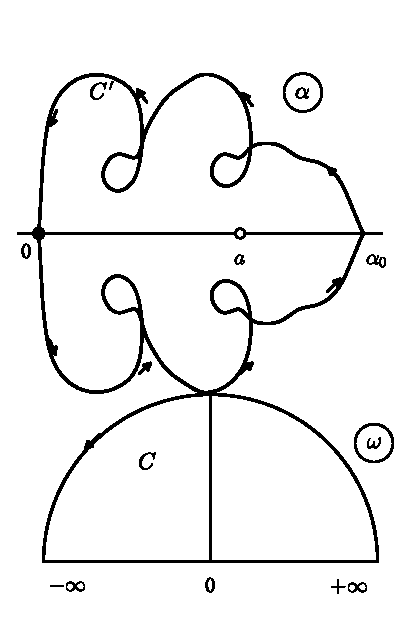
\includegraphics[width=6.5cm]{fig53.pdf}\\[0.3em]{\small 图 53}\end{minipage}\par\nopagebreak

为了计算积分，我们把它写成形式
\begin{equation*}
  \frac{1}{2\pi\mathrm{i}}\int_{C'}\frac{\mathrm{d}\alpha}{\alpha-a},
\end{equation*}
这时积分沿复变量 $\alpha$ 平面中的围道 $C'$,围道 $C'$ 是 $\omega$ 平面中围道 C 的映像.整个无限大半圆映像到 $\alpha=0$ 这一点，而坐标原点 $(\omega=0)$ 映像到另一实数点 $\alpha_0$. $\omega$ 的正、负两半实轴映像到 $\alpha$ 平面中非常复杂的(一般是自交的)两条曲线，分别整条落在上、下两半平面内.重要的是：这两条曲线除了在 $\alpha=0$ 和 $\alpha=\alpha_0$ 两点以外不与横坐标轴在任何一点相交，因为在 $\omega$ 为任何有限实值($\omega=0$ 除外)时，$\alpha$ 都不取实值.由于围道 $C'$ 具有这种性质，如果 $a$ 点是位于0和 $\alpha_0$ 之间(如图53所示），那么当复数 $\alpha-a$ 沿着围道 $C'$ 环绕一周时其辐角的总改变等于 $2\pi$；如果a位于该区间以外，那么总改变等于 $0$，与围道的自相交次数无关.因此(123.13)式在 $0<a<\alpha_0$ 时等于1,在a的其它任何值下则等于0.

于是我们得出结论：在 $\omega$ 的上半平面，对于位于上述区间内的任何实数值 $a,\alpha(\omega)$ 只取一次(而对区间以外的任何实数值，$\alpha(\omega)$ 一次也不取). 由此我们首先可以推断：在函数 $\alpha(\omega)$ 为实数的虚轴上，它不能具有极大值，也不能有极小值，否则它就会至少两次取某些值.因此在虚轴上函数 $\alpha(\omega)$ 单调地变化，对于从 $\alpha_0$ 到0的所有实数值，只在虚轴上取而不在任何别处，并且只取一次.

如果 $\alpha_0=\infty$(即 $\alpha(\omega)$ 在 $\omega=0$ 有极点），那么上述的证明只需改动如下：(在 $\omega$ 平面内)围道沿实轴部分应走原点上方的一个无穷小半圆绕开原点.这时图 53 中的围道 $C'$ 的改变，可以设想成把 $\alpha_0$ 移到无穷远去的结果.这种情形下，在虚轴上函数 $\alpha(\omega)$ 单调地从 $+\infty$ 减小到零.

现在我们来推导函数 $\alpha(\omega)$ 的实部和虚部的一个关系式.为此，我们选取任意正实值 $\omega=\omega_0$ 然后沿图54中所示的围道积分 $\frac{\alpha}{\omega-\omega_0}$.这个围道沿整个实轴走，而从点 $\omega=\omega_0>0$(可能还有点 $\omega=0$,如果它是函数 $\alpha(\omega)$ 的极点)的上方绕开.这个围道由一个无穷大的半圆来闭合.在无穷远处，$\alpha\to 0$,因而函数 $\frac{\alpha}{\omega-\omega_0}$ 比 $\frac{1}{\omega}$ 更快地趋于0.因此以下积分收敛：
\begin{equation*}
  \int_C\frac{\alpha(\omega)}{\omega-\omega_0}\,\mathrm{d}\omega;
\end{equation*}
$\alpha(\omega)$ 在上半平面内没有奇点，而 $\omega=\omega_0$ 这一点已被排除在积分区域以外，因此函数 $\frac{\alpha}{\omega-\omega_0}$ 在围道C内处处解析，于是该积分等于零.

\par\nopagebreak\noindent\begin{minipage}{\linewidth}\centering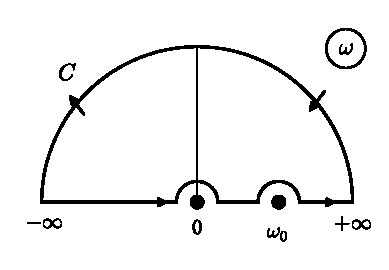
\includegraphics[width=5cm]{fig54.pdf}\\[0.3em]{\small 图 54}\end{minipage}\par\nopagebreak

沿无穷远半圆的积分本身也等于零.点 $\omega_0$ 由一个无穷小半圆(半径 $\rho\to 0$)绕开.积分回路方向沿顺时针，因此对积分的贡献等于 $-\mathrm{i}\pi\alpha(\omega_0)$.如果 $\alpha_0$ 有限，不必绕开原点，因此沿整个实轴的积分为：
\begin{equation*}
  \lim_{\rho\to 0}\left\{\int_{-\infty}^{\omega_0-\rho}
  \frac{\alpha}{\omega-\omega_0}\,\mathrm{d}\omega
  +\int_{\omega_0+\rho}^{\infty}\frac{\alpha}{\omega-\omega_0}\,\mathrm{d}\omega\right\}
  -\mathrm{i}\pi\alpha(\omega_0)=0.
\end{equation*}
第一项是从 $-\infty$ 到 $+\infty$ 的积分主值.用通常记号表示主值，于是有：
\begin{equation}
  \mathrm{i}\pi\alpha(\omega_0)
  =\mathrm{P}\int_{-\infty}^{\infty}\frac{\alpha}{\omega-\omega_0}\,\mathrm{d}\omega.
\end{equation}
在这里积分变量 $\omega$ 只取实数值.改用字母 $\xi$ 来取代 $\omega$,而用 $\omega$ 取代给定的实数值 $\omega_0$;并且实变量 $\omega$ 的函数 $\alpha(\omega)$ 也写成 $\alpha=\alpha'+\mathrm{i}\alpha''$ 的形式.取(123.14)的实部和虚部，最后求出下列两个关系式：
\begin{equation}
  \alpha'(\omega)=\frac{1}{\pi}\mathrm{P}\int_{-\infty}^{\infty}
  \frac{\alpha''(\xi)}{\xi-\omega}\,\mathrm{d}\xi,
\end{equation}
\begin{equation}
  \alpha''(\omega)=-\frac{1}{\pi}\mathrm{P}\int_{-\infty}^{\infty}
  \frac{\alpha'(\xi)}{\xi-\omega}\,\mathrm{d}\xi.
\end{equation}
这两个关系式(称为色散关系)首先由克拉默斯和克勒尼希(H.A.Kramers,R.L. Kronig,1927)得出. 应当强调：在推导关系式时所用到的函数 $\alpha(\omega)$ 的唯一重要性质只是上半平面无奇点\footnote{至于$\omega\to\infty$时$\alpha\to0$的假设则是无关紧要的：假如极限$\alpha_\infty$不等于零，那么只需以差$\alpha-\alpha_\infty$代替$\alpha$，并在公式(123.15)，(123.16)中作相应的显而易见的改动.另见§126的习题.}.因此可以说：克拉默斯-克勒尼希公式就像函数 $\alpha(\omega)$ 描述过的性质一样，是因果性物理原理的直接结果.

$\alpha''(\xi)$ 是奇函数，利用这一点，我们也可以把(123.15)改写成形式
\begin{equation*}
  \alpha'(\omega)=\frac{1}{\pi}\mathrm{P}\int_0^{\infty}
  \frac{\alpha''(\xi)}{\xi-\omega}\,\mathrm{d}\xi
  +\frac{1}{\pi}\mathrm{P}\int_0^{\infty}
  \frac{\alpha''(\xi)}{\xi+\omega}\,\mathrm{d}\xi,
\end{equation*}
即
\begin{equation}
  \alpha'(\omega)=\frac{2}{\pi}\mathrm{P}\int_0^{\infty}
  \frac{\xi\alpha''(\xi)}{\xi^2-\omega^2}\,\mathrm{d}\xi.
\end{equation}
如果函数 $\alpha(\omega)$ 在 $\omega=0$ 点有极点，而在它附近 $\alpha=\frac{\mathrm{i}A}{\omega}$,那么绕开极点的半圆回路给出附加的实数项 $-\frac{A}{\omega}$,它应加到等式(123.14)的左边.因此这一项也出现在(123.16)式中：
\begin{equation}
  \alpha''(\omega)=-\frac{1}{\pi}\mathrm{P}\int_{-\infty}^{\infty}
  \frac{\alpha'(\xi)}{\xi-\omega}\,\mathrm{d}\xi+\frac{A}{\omega};
\end{equation}
但是关系式(123.15)或(123.17)则保持不变.

我们也可以推导出一个关系式用实轴上的 $\alpha''(\omega)$ 值来表示正虚轴上的 $\alpha(\omega)$ 值.为此，我们考虑积分
\begin{equation*}
  \int\frac{\omega\alpha(\omega)}{\omega^2+\omega_0^2}\,\mathrm{d}\omega,
\end{equation*}
围道取实轴和上半平面的无穷大半圆 ($\omega_0$ 为一实数). 这个积分可以用被积式在极点 $\omega=\mathrm{i}\omega_0$ 的留数表示.另一方面，沿无穷大半圆的积分等于零，因此我们求出：
\begin{equation*}
  \int_{-\infty}^{\infty}\frac{\omega\alpha(\omega)}{\omega^2+\omega_0^2}\,\mathrm{d}\omega
  =\mathrm{i}\pi\alpha(\mathrm{i}\omega_0).
\end{equation*}
由于被积式是奇函数，等式左边积分实部为零.再把符号 $\omega_0$ 改成 $\omega$,把 $\omega$ 改成 $\xi$,最后得到
\begin{equation}
  \alpha(\mathrm{i}\omega)=\frac{2}{\pi}\int_0^{\infty}
  \frac{\xi\alpha''(\xi)}{\omega^2+\xi^2}\,\mathrm{d}\xi.
\end{equation}
上式两边对 dω积分，得
\begin{equation}
  \int_0^{\infty}\alpha(\mathrm{i}\omega)\,\mathrm{d}\omega
  =\int_0^{\infty}\alpha''(\omega)\,\mathrm{d}\omega.
\end{equation}

\section{涨落耗散定理}

现在我们进一步计算，以便将涨落量x与上节引进的广义响应率相联系.

设变量x所属的物体处于某个确定的(第n个)定态.平均值(122.8)可以作为以下算符的相应的对角矩阵元来计算
\begin{equation}
  \frac{1}{2}\left(\hat{x}_\omega\hat{x}_{\omega'}
  +\hat{x}_{\omega'}\hat{x}_\omega\right)_{nn}
  =\frac{1}{2}\sum_m\left[(x_\omega)_{nm}(x_{\omega'})_{mn}
  +(x_{\omega'})_{nm}(x_\omega)_{mn}\right],
\end{equation}
式中求和遍及整个能谱(由于 $\hat{x}_\omega$ 是复算符，方括号中的两项彼此不等).

算符 $\hat{x}(t)$ 依赖于时间，这意味着在计算其矩阵元时必须使用含时波函数.因此有
\begin{equation}
  (x_\omega)_{nm}=\int_{-\infty}^{\infty}x_{nm}
  \mathrm{e}^{\mathrm{i}(\omega_{nm}+\omega)t}\,\mathrm{d}t
  =2\pi x_{nm}\delta(\omega_{nm}+\omega),
\end{equation}
式中 $x_{nm}$ 是通常用物体粒子坐标表示的算符x的不含时矩阵元，而
$\omega_{nm}=\dfrac{E_n-E_m}{\hbar}$ 是状态n和状态m之间跃迁的频率.由此可见
\begin{equation*}
\begin{aligned}
  \frac{1}{2}\left(\hat{x}_\omega\hat{x}_{\omega'}
  +\hat{x}_{\omega'}\hat{x}_\omega\right)_{nn}&=\\
  &=2\pi^2\sum_m|x_{nm}|^2\left[\delta(\omega_{nm}+\omega)\delta(\omega_{mn}+\omega')
  +\delta(\omega_{nm}+\omega')\delta(\omega_{mn}+\omega)\right]
\end{aligned}
\end{equation*}
(在这里已经考虑到，由于x是实数，$x_{nm}=x_{mn}^*$).在方括号中的δ函数的乘积显然可以改写成
\begin{equation*}
  \delta(\omega_{nm}+\omega)\delta(\omega+\omega')
  +\delta(\omega_{mn}+\omega)\delta(\omega+\omega').
\end{equation*}
然后再与(122.8)相比较，我们得到下式
\begin{equation}
  (x^2)_\omega=\pi\sum_m|x_{nm}|^2\left[\delta(\omega+\omega_{nm})
  +\delta(\omega+\omega_{mn})\right].
\end{equation}
关于这个表达式的写法，我们作如下说明.虽然宏观物体的能级严格地讲是分立的，但是它们相当稠密，以至于实际上形成连续谱.如果把公式(124.3)对频率的小间隔(仍含很多能级)平均，那么可以不用δ函数把它写出.如果 $\Gamma(E)$ 是能量小于E的能级数，则
\begin{equation}
  (x^2)_\omega=\pi\hbar|x_{nm}|^2\left(\frac{\mathrm{d}\Gamma}{\mathrm{d}E_m}
  +\frac{\mathrm{d}\Gamma}{\mathrm{d}E_m'}\right),
\end{equation}
式中 $E_m=E_n+\hbar\omega,\ E_m'=E_n-\hbar\omega$.

现在假设有一个由以下算符描述的(频率为ω的)周期微扰作用在物体上：
\begin{equation}
  \hat{V}=-f\hat{x}=-\frac{1}{2}\left(f_0\mathrm{e}^{-\mathrm{i}\omega t}
  +f_0^*\mathrm{e}^{\mathrm{i}\omega t}\right)\hat{x}.
\end{equation}
在这个微扰的影响下，系统(在单位时间内)发生跃迁n→m的概率如下式：
\begin{equation}
  w_{mn}=\frac{\pi|f_0|^2}{2\hbar^2}|x_{mn}|^2
  \left[\delta(\omega+\omega_{mn})+\delta(\omega+\omega_{nm})\right]
\end{equation}
(参看第三卷§42).这个公式中的两项分别由(124.5)中的两项产生.在每次跃迁中系统吸收(或发射)一个量子 $\hbar\omega$. 和式
\begin{equation*}
  Q=\sum_m w_{mn}\hbar\omega_{mn}
\end{equation*}
给出物体(单位时间内)所吸收的平均能量；这个能量来源是外部微扰，物体吸收后，耗散在物体中.把(124.6)代入上式，我们得到
\begin{equation*}
  Q=\frac{\pi}{2\hbar}|f_0|^2\sum_m|x_{nm}|^2
  \left[\delta(\omega+\omega_{mn})+\delta(\omega+\omega_{nm})\right]\omega_{mn}
\end{equation*}
或者，考虑到δ函数仅在其宗量为零时才不等于零，
\begin{equation}
  Q=\frac{\pi}{2\hbar}\omega|f_0|^2\sum_m|x_{nm}|^2
  \left[\delta(\omega+\omega_{nm})-\delta(\omega+\omega_{mn})\right].
\end{equation}
把(124.7)与(123.11)相比较，我们求出
\begin{equation}
  \alpha''(\omega)=\frac{\pi}{\hbar}\sum_m|x_{nm}|^2
  \left[\delta(\omega+\omega_{nm})-\delta(\omega+\omega_{mn})\right].
\end{equation}
用这种方法算出的 $(x^2)_\omega$ 和 $\alpha''$ 这两个量之间以一个简单的关系相联.但是，只有在这两个量用物体的温度写下以后，这个关系式才显现出来.为此，我们借助于吉布斯分布求平均(参看§118第一个脚注).对于 $(x^2)_\omega$ 我们有
\begin{equation*}
  (x^2)_\omega=\pi\sum_{n,m}\rho_n|x_{nm}|^2
  \left[\delta(\omega+\omega_{nm})+\delta(\omega+\omega_{mn})\right],
\end{equation*}
式中为简便起见记
\begin{equation*}
  \rho_n=\exp\frac{F-E_n}{T},
\end{equation*}
$E_n$ 是物体的能级，F是物体的自由能.因为现在求和对两个指标m和n进行，所以可以置换指标.去掉方括号，并在第二项中置换m和n，得到
\begin{equation*}
\begin{aligned}
  (x^2)_\omega&=\pi\sum_{m,n}(\rho_n+\rho_m)|x_{nm}|^2\delta(\omega+\omega_{nm})\\
  &=\pi\sum_{m,n}\rho_n(1+\mathrm{e}^{\hbar\omega_{nm}/T})|x_{nm}|^2
  \delta(\omega+\omega_{nm})
\end{aligned}
\end{equation*}
或者，由于和式中的δ函数
\begin{equation*}
  (x^2)_\omega=\pi(1+\mathrm{e}^{-\hbar\omega/T})\sum_{m,n}\rho_n|x_{nm}|^2
  \delta(\omega+\omega_{nm}).
\end{equation*}
用完全类似的方法可得到
\begin{equation*}
  \alpha''=\frac{\pi}{\hbar}(1-\mathrm{e}^{-\hbar\omega/T})\sum_{m,n}\rho_n|x_{nm}|^2
  \delta(\omega+\omega_{nm}).
\end{equation*}
这两个式子相互比较，求出
\begin{equation}
  (x^2)_\omega=\hbar\alpha''\coth\frac{\hbar\omega}{2T}
  =2\hbar\alpha''\left\{\frac{1}{2}
  +\frac{1}{\mathrm{e}^{\hbar\omega/T}-1}\right\}.
\end{equation}
涨落量的总均方值由积分给出：
\begin{equation}
  \langle x^2\rangle=\frac{\hbar}{\pi}\int_0^{\infty}\alpha''(\omega)
  \coth\frac{\hbar\omega}{2T}\,\mathrm{d}\omega.
\end{equation}
这些重要的公式构成涨落耗散定理(简记为FDT)的内容，由Callen和 Welton(H. B. Callen，T. A. Welton，1951)提出. 这些公式把系统在外部微扰作用下物理量的涨落与耗散性质联系起来.我们注意到:在(124.9)中括号内的因子是在温度 T下振子的平均能量(以 $\hbar\omega$为单位)；$\frac{1}{2}$ 那一项对应于零点振动.

与§118最后所作的完全类似，所得到的这些结果可以表示成另一种形式，只要形式地设想量x的自发涨落来自某种虚拟随机力的作用.在这种情况下，写公式用傅里叶分量 $x_\omega$ 和 $f_\omega$,并处理x如经典量，比较方便.它们之间的关系类似于(123.3),为
\begin{equation}
  x_\omega=\alpha(\omega)f_\omega,
\end{equation}
此后，对于均方涨落有
\begin{equation*}
  \left\langle x_\omega x_{\omega'}\right\rangle
  =\alpha(\omega)\alpha(\omega')\left\langle f_\omega f_{\omega'}\right\rangle,
\end{equation*}
或者，按照定义(122.4)，转换为涨落的谱密度：
\begin{equation*}
  (x^2)_\omega=\alpha(\omega)\alpha(-\omega)(f^2)_\omega
  =|\alpha(\omega)|^2(f^2)_\omega,
\end{equation*}
因此，由(124.9)求出随机力的均方值的谱密度为
\begin{equation}
  (f^2)_\omega=\frac{\hbar\alpha''(\omega)}{|\alpha(\omega)|^2}
  \coth\frac{\hbar\omega}{2T}.
\end{equation}
这种处理方法在理论的具体应用中有些优点.

涨落耗散定理的推导基于把外界作用(124.5)看成小扰动；系统响应是线性的，即 $\bar{x}$ 与力 $f$ 之间线性关联，这也与作用很小有关.但是，应该强调，这不会导致对x这个量平均涨落的准许值本身产生任何物理限制.只要辅助量f足够小，就可以保证外部作用很小，而f不在涨落耗散定理的最后表达式中出现.因此，对于所考虑的物理量x的类型，它们(在热力学平衡的系统内)涨落的性质，完全取决于系统对无论多弱的外来作用如何响应的性质.

在 $T\gg\hbar\omega$ 的温度下,$\coth(\hbar\omega/2T)\approx 2T/\hbar\omega$,公式(124.9)变成
\begin{equation}
  (x^2)_\omega=\frac{2T}{\omega}\alpha''(\omega).
\end{equation}
其中量子常数消失，这相应于在这些条件下涨落是经典的.

如果对于所有主要的频率(那里 $\alpha''(\omega)$ 明显非零)不等式 $T\gg\hbar\omega$ 都成立，则在积分公式(124.10)中也可以取经典极限：
\begin{equation*}
  \langle x^2\rangle=\frac{2T}{\pi}\int_0^{\infty}\frac{\alpha''(\omega)}{\omega}\,\mathrm{d}\omega.
\end{equation*}
但是根据(123.17)，这个积分可以用静态值 $\alpha'(0)=\alpha(0)$ 表示，因此\footnote{这个表达式也能从经典统计的吉布斯分布直接得到.设$x=x(q,p)$是某个经典量.在系统的能量中引入一项$xf$($f$为常数)，对于平均值$\bar{x}$，我们有
\begin{equation*}
  \bar{x}=\int x(p,q)\exp\frac{F-E(q,p)+x(q,p)f}{T}\,\mathrm{d}q\,\mathrm{d}p.
\end{equation*}
按照定义$f\to0$时$\alpha(0)=\mathrm{d}\bar{x}/\mathrm{d}f$；对上式取微商，求得
\begin{equation*}
  \alpha(0)=\frac{1}{T}\int x^2\exp\frac{F-E}{T}\,\mathrm{d}q\,\mathrm{d}p=\frac{1}{T}\langle x^2\rangle
\end{equation*}
(自由能$F$也依赖于$f$，但是，在令$f=0$，即$\bar{x}=0$之后，含导数$\frac{\partial F}{\partial f}$的一项消失).}
\begin{equation}
  \langle x^2\rangle=T\alpha(0).
\end{equation}
最后，我们回到以上结果与准定态涨落理论(§118)的联系.

首先我们注意到，如果x这个量具有在§110中所指的小涨落(即容许熵作展开(110.3))，则平方平均 $\langle x^2\rangle=1/\beta$.与(124.14)相比较表明，对于这样的量，
\begin{equation}
  \alpha(0)=\frac{1}{\beta T}.
\end{equation}
其次，设x属于具有准定态涨落的一类量.假定物体受到静止力f的作用.这使得平衡态移动到x已不再为零而等于 $\tilde{x}=\alpha(0)f=f/\beta T$ 的状态.于是描述远离平衡态系统弛豫的宏观方程形式为
\begin{equation}
  \dot{x}=-\lambda\left(x-\frac{f}{\beta T}\right),
\end{equation}
它与方程(118.5) $\dot{x}=-\lambda x$ 的区别在于速率 $\dot{x}$ 不是在 $x=0$ 处变为零，而是在 $x=f/\beta T$ 处.

可以认为方程(124.16)在物体受到含时的微扰作用时仍适用，只要力 $f(t)$ 变化的周期比非完全平衡(对应于给定的x值)的建立时间大得多.如果f(t)是频率为 $\omega$ 的时间周期函数，则宏观值 $x(t)$ 也以同样的频率变化.把形为(123.8),(123.9)的 $f(t)$、$\bar{x}(t)$ 代入方程(124.16),并从中分出含 $\exp(-\mathrm{i}\omega t)$ 和 $\exp(\mathrm{i}\omega t)$ 的项，得
\begin{equation*}
  -\mathrm{i}\omega\alpha(\omega)f_0
  =-\lambda\alpha(\omega)f_0+\frac{\lambda}{\beta T}f_0,
\end{equation*}
由此得出
\begin{equation}
  \alpha(\omega)=\frac{\lambda}{\beta T(\lambda-\mathrm{i}\omega)}.
\end{equation}
根据涨落耗散定理(124.9),现在求出
\begin{equation}
  (x^2)_\omega=\frac{2\lambda}{\beta(\lambda^2+\omega^2)}
  \frac{\hbar\omega}{2T}\coth\frac{\hbar\omega}{2T}.
\end{equation}
这个结果推广了适用于经典量涨落的公式(122.9).表达式(124.18)与(122.9)差一个因子
\begin{equation}
  \frac{\hbar\omega}{2T}\coth\frac{\hbar\omega}{2T},
\end{equation}
它在 $\hbar\omega\ll T$ 的经典极限下变为1.

方程(124.16)也可以用另一种方式理解：不把它看成(处于外部作用下的)远离平衡系统的宏观运动方程，而看成在随机力f作用下平衡闭合系统内 $x(t)$ 这个量的涨落方程.在这种解释下，它对应于方程(118.9)，因此随机力的两种定义差别只在因子 $y=\frac{\lambda f}{T\beta}$.把(124.17)代入(124.12)，我们求出谱密度 $(y^2)_\omega$ 为
\begin{equation}
  (y^2)_\omega=\frac{2\lambda}{\beta}\frac{\hbar\omega}{2T}
  \coth\frac{\hbar\omega}{2T},
\end{equation}
它与原来的表达式(122.10)相差一个同样的因子(124.19).

\section{多个量的涨落耗散定理}

涨落耗散定理可以很容易地推广到同时有多个涨落量 $x_i$ 的情形.

在这种情形下广义响应率取决于系统对如下形式微扰的响应：
\begin{equation}
  \hat{V}=-\hat{x}_if_i(t),
\end{equation}
而且它们就是平均值 $\bar{x}_i(t)$ 与广义力 $f_i(t)$ 的傅里叶分量之间线性关系中的系数：
\begin{equation}
  \bar{x}_{i\omega}=\alpha_{ik}(\omega)f_{k\omega}.
\end{equation}
系统能量的变化根据下式用外部微扰表示：
\begin{equation}
  \dot{E}=-\dot{f}_i\bar{x}_i.
\end{equation}
就像公式(123.10)一样，该式通常用于建立量 $x_i$ 和 $f_i$ 之间的实际对应关系，作为理论的具体应用.

涨落的谱密度用如下的对称化乘积算符的平均值引入：
\begin{equation}
  \frac{1}{2}\left\langle\hat{x}_{i\omega}\hat{x}_{k\omega'}
  +\hat{x}_{k\omega'}\hat{x}_{i\omega}\right\rangle
  =2\pi(x_ix_k)_\omega\delta(\omega+\omega'),
\end{equation}
该式是(122.8)式的推广.这个平均值的计算，完全类似于(124.3)的推导，就是计算矩阵的对角(nn)元，结果为
\begin{equation}
  (x_ix_k)_\omega=\pi\sum_m\left[(x_i)_{nm}(x_k)_{mn}\delta(\omega+\omega_{nm})
  +(x_k)_{nm}(x_i)_{mn}\delta(\omega+\omega_{mn})\right].
\end{equation}
设周期性微扰作用于系统，在该微扰中
\begin{equation}
  f_i(t)=\frac{1}{2}\left(f_{0i}\mathrm{e}^{-\mathrm{i}\omega t}
  +f_{0i}^*\mathrm{e}^{\mathrm{i}\omega t}\right).
\end{equation}
系统对该微扰的响应为
\begin{equation}
  \bar{x}_i(t)=\frac{1}{2}\left[\alpha_{ik}(\omega)f_{0k}\mathrm{e}^{-\mathrm{i}\omega t}
  +\alpha_{ik}^*(\omega)f_{0k}^*\mathrm{e}^{\mathrm{i}\omega t}\right].
\end{equation}
把(125.6)，(125.7)代入(125.3)并按微扰的一个周期求平均，代替(123.11)，我们得到耗散能量的如下表达式：
\begin{equation}
  Q=\frac{\mathrm{i}\omega}{4}(\alpha_{ik}^*-\alpha_{ki})f_{0i}f_{0k}^*.
\end{equation}
另一方面，与推导(124.7)相似的计算给出
\begin{equation*}
  Q=\frac{\pi}{2\hbar}\omega\sum_m f_{0i}f_{0k}^*
  \left[(x_i)_{mn}(x_k)_{nm}\delta(\omega+\omega_{nm})
  -(x_i)_{nm}(x_k)_{mn}\delta(\omega+\omega_{mn})\right],
\end{equation*}
与(125.8)相比较，我们得到
\begin{equation}
  \alpha_{ik}^*-\alpha_{ki}=-\frac{2\pi\mathrm{i}}{\hbar}\sum_m
  \left[(x_i)_{mn}(x_k)_{nm}\delta(\omega+\omega_{nm})
  -(x_i)_{nm}(x_k)_{mn}\delta(\omega+\omega_{mn})\right].
\end{equation}
最后，把(125.5)和(125.9)按吉布斯分布求平均如上节，我们求出涨落耗散定理(124.9)的如下推广公式：
\begin{equation}
  (x_ix_k)_\omega=\frac{1}{2}\mathrm{i}\hbar(\alpha_{ki}^*-\alpha_{ik})
  \coth\frac{\hbar\omega}{2T}.
\end{equation}
与(124.11)，(124.12)式相似，也可以把(125.10)用虚拟的随机力来表示，随机力的作用给出的结果与 $x_i$ 这些量的自发涨落完全等效.为此，我们写出
\begin{equation}
  x_{i\omega}=\alpha_{ik}f_{k\omega},\qquad
  f_{i\omega}=\alpha^{-1}_{ik}x_{k\omega}
\end{equation}
进而有
\begin{equation*}
  (f_if_k)_\omega=\alpha^{-1}_{il}\alpha^{-1}_{km}(x_lx_m)_\omega.
\end{equation*}
把(125.10)代入上式，就得到
\begin{equation}
  (f_if_k)_\omega=\frac{\mathrm{i}\hbar}{2}
  (\alpha^{-1}_{ik}-\alpha^{-1*}_{ki})\coth\frac{\hbar\omega}{2T}.
\end{equation}
所得到的这些结果使我们能够作出一些有关广义响应率 $\alpha_{ik}(\omega)$ 对称性质的结论(H. B. Callen,M. L. Barrash,J. L. Jackson,R. F. Green,1952). 首先，我们假设 $x_i, x_k$ 这些量在时间反演下不变；那么它们对应的算符 $\hat{x}_i, \hat{x}_k$ 是实的.此外，我们还认为物体不具有磁结构(参看§128第一个脚注)，也不处于外磁场中;那么其定态波函数也是实的\footnote{相互作用粒子系统的精确能级只可能相对于系统的总角动量取向是简并的.假设物体包在器壁不动的容器内，可以消除简并的这种来源.此后物体的能级就是非简并的，因而与此相应的精确波函数可以选为实的.}.因此x的矩阵元也是实的，而考虑到矩阵 $x_{nm}$ 的厄米性，我们有 $x_{nm}=x_{mn}^*=x_{mn}$.那么等式(125.9)的右边对于指标i,k是对称的，因而左边对于指标i,k也是对称的.这样，$\alpha_{ik}^*-\alpha_{ki}=\alpha_{ki}^*-\alpha_{ik}$,或者 $\alpha_{ik}+\alpha_{ik}^*=\alpha_{ki}+\alpha_{ki}^*$，也就是说，我们得出结论：$\alpha_{ik}$ 的实部是对称的.

但是每个 $\alpha_{ik}$ 的实部 $(\alpha'_{ik})$ 和虚部 $(\alpha''_{ik})$ 都由线性积分关系即克拉默斯-克勒尼希公式相联系.所以从 $\alpha'_{ik}$ 的对称性也得出 $\alpha''_{ik}$ 的对称性，因而有整个 $\alpha_{ik}$ 的对称性.因此，我们得到最后结果：
\begin{equation}
  \alpha_{ik}(\omega)=\alpha_{ki}(\omega).
\end{equation}
如果物体处于外磁场H中，这些关系式的形式有些变化.在外磁场中系统的波函数不是实的，但具有性质 $\psi^*(\boldsymbol{H})=\psi(-\boldsymbol{H})$. 相应地对于x的矩阵元，我们有
\begin{equation*}
  x_{nm}(\boldsymbol{H})=x_{mn}(-\boldsymbol{H}),
\end{equation*}
并且在交换指标i,k时，只有同时也改变磁场H的符号，(125.9)右边的表达式才不改变.因此我们得到关系式
\begin{equation*}
  \alpha_{ik}^*(\boldsymbol{H})-\alpha_{ki}(\boldsymbol{H})
  =\alpha_{ik}^*(-\boldsymbol{H})-\alpha_{ki}(-\boldsymbol{H}).
\end{equation*}
根据由克拉默斯-克勒尼希公式(123.14)给出的另一个关系式，可以得出 $\alpha_{ki}=\mathrm{i}\hat{J}(\alpha_{ki})$,式中 $\hat{J}$ 是实线性算符.把这个等式与厄米共轭等式 $\alpha_{ik}^*=-\mathrm{i}\hat{J}(\alpha_{ik}^*)$ 相加，得到
\begin{equation*}
  \alpha_{ik}^*+\alpha_{ki}=-\mathrm{i}\hat{J}(\alpha_{ik}^*-\alpha_{ki})
\end{equation*}
(在式中，所有的 $\alpha_{ik}$ 当然有同样的H值).由此看出：如果差 $\alpha_{ik}^*-\alpha_{ki}$ 具有某种对称性，则和 $\alpha_{ik}^*+\alpha_{ki}$ 也同样具有，因而量 $\alpha_{ik}$ 本身也同样.因此，
\begin{equation}
  \alpha_{ik}(\omega;\boldsymbol{H})
  =\alpha_{ki}(\omega;-\boldsymbol{H}).
\end{equation}
最后，假设x这些量中有一些在时间反演下变号.这样的量的算符是纯虚的，因此 $x_{nm}=x_{mn}^*=-x_{mn}$.如果 $x_i, x_k$ 两个量都属于这种类型，则全部推导和(125.13)的结果保持不变.假如这两个量中有一个在时间反演下变号，则在交换指标i,k时，等式(125.9)的右边变号.相应地，(125.13)变为
\begin{equation}
  \alpha_{ik}(\omega)=-\alpha_{ki}(\omega),
\end{equation}
或者，对于磁场中的物体，有
\begin{equation}
  \alpha_{ik}(\omega;\boldsymbol{H})
  =-\alpha_{ki}(\omega;-\boldsymbol{H}).
\end{equation}
当然，所有这些关系式也可以作为涨落的时间对称性的结果而由(125.10)式得出.这样，如果 $x_i$ 和 $x_k$ 这两个量时间反演行为相同，则由于所述的对称性 $(x_ix_k)_\omega$ 是实的，并且相对于指标i,k对称(参看§122).于是公式(125.10)的右边对于同样的指标也必须是对称的，我们再次得出结果(125.13).广义响应率对称性质的这种推导与§120中动理学系数对称性原理的推导完全相似；下面将看到，公式(125.13)—(125.16)可以看成这个原理的推广.

广义响应率与动理学系数的联系可以通过把涨落耗散定理与多变量准定态涨落理论相比来说明.我们写出这些相对应的公式，不再重复与上节末尾讨论单变量情况相似的所有内容.

响应率的静态值与熵的展开系数 $\beta_{ik}$ 由如下等式相联系
\begin{equation*}
  T\alpha_{ik}(0)=\beta^{-1}_{ik}.
\end{equation*}
因此系统在静态力 $f_k$ 作用下对平衡状态的偏移的决定量为
\begin{equation*}
  \bar{x}_i=\alpha_{ik}(0)f_k=\frac{\beta^{-1}_{ik}f_k}{T},\qquad
  \bar{X}_i=\beta_{ik}\bar{x}_k=\frac{f_i}{T}.
\end{equation*}
准静态力 $f_k(t)$ 作用下非平衡系统的宏观运动方程可以表示成
\begin{equation}
  \dot{x}_i=-\gamma_{ik}\left(X_k-\frac{f_k}{T}\right),
\end{equation}
它与(120.5)不同之处在于用 $X_k-\dfrac{f_k}{T}$ 代替了 $X_k$.

把形为周期函数(125.6)，(125.7)的 $x_i(t)$ 和 $f_i(t)$ 代入(125.17)（并且把 $X_k$ 写成线性组合 $X_k=\beta_{kl}x_l$ 的形式），我们得到
\begin{equation*}
  -\mathrm{i}\omega\alpha_{im}f_{0m}
  =-\gamma_{ik}\beta_{kl}\alpha_{lm}f_{0m}+\frac{1}{T}\gamma_{im}f_{0m},
\end{equation*}
由于 $f_{0m}$ 的任意性，由此得出这些系数之间的关系式
\begin{equation*}
  -\mathrm{i}\omega\alpha_{im}+\gamma_{ik}\beta_{kl}\alpha_{lm}
  =\frac{1}{T}\gamma_{im},
\end{equation*}
或
\begin{equation}
  \alpha_{ik}=\frac{1}{T}(\beta-\mathrm{i}\omega\gamma^{-1})^{-1}_{ik}.
\end{equation}
这就建立起所求的 $\alpha_{ik}$ 与动理学系数 $\gamma_{ik}$ 之间的联系.

按照定义 $\beta_{ik}$ 相对于自己的两个指标是对称的(作为导数 $-\dfrac{\partial^2 S}{\partial x_i\partial x_k}$).因此由 $\alpha_{ik}$ 的对称性也就得出 $\gamma_{ik}$ 的对称性，即通常的动理学系数的对称性原理.

在方程(125.17)中把 $f_k$ 看成随机力，把(125.18)代入(125.12)中我们得到
\begin{equation*}
  (f_if_k)_\omega=\frac{1}{2}\hbar\omega T
  (\gamma^{-1}_{ik}+\gamma^{-1}_{ki})\coth\frac{\hbar\omega}{2T}.
\end{equation*}
如果像(122.20)那样定义随机力 $y_i$,则 $y_i=\gamma_{ik}f_k/T$;对于它们的谱分布有
\begin{equation}
  (y_iy_k)_\omega=(\gamma_{ik}+\gamma_{ki})\frac{\hbar\omega}{2T}
  \coth\frac{\hbar\omega}{2T}.
\end{equation}
这个表达式与(122.21)差一同样的因子(124.19)，在经典极限下它变为1.

\section{广义响应率的算符形式}

涨落耗散定理也可以倒过来看，把等式(124.9)从右边读到左边，并且把 $(x^2)_\omega$ 以显式写成关联函数的傅里叶分量：
\begin{equation}
  \alpha''(\omega)=\frac{1}{2\hbar}\tanh\frac{\hbar\omega}{2T}
  \int_{-\infty}^{\infty}\mathrm{e}^{\mathrm{i}\omega t}
  \left\langle\hat{x}(0)\hat{x}(t)+\hat{x}(t)\hat{x}(0)\right\rangle\mathrm{d}t.
\end{equation}
在这种形式下，该公式表明原则上能够根据系统的微观性质计算出系数 $\alpha''(\omega)$.但是其不足之处在于它只能直接确定 $\alpha(\omega)$ 的虚部，而不是整个函数.可以得到没有这种缺点的类似公式.为此，我们对微扰系统直接计算量子力学平均值 $\bar{x}$(用微扰算符(124.5)\footnote{这种方法比使用克拉默斯-克勒尼希关系式根据$\alpha''(\omega)$来决定$\alpha'(\omega)$(然后再决定整个$\alpha(\omega)$)更加直接.}).

设 $\Psi_n^{(0)}$ 是未微扰系统的波函数.我们按照普遍的方法(参看第三卷§40)，求微扰系统的一级近似波函数，
\begin{equation}
  \Psi_n=\Psi_n^{(0)}+\sum_ma_{mn}\Psi_m^{(0)},
\end{equation}
式中系数 $a_{mn}$ 满足方程
\begin{equation*}
  \mathrm{i}\hbar\frac{\mathrm{d}a_{mn}}{\mathrm{d}t}
  =V_{mn}\mathrm{e}^{\mathrm{i}\omega_{mn}t}
  =-\frac{1}{2}x_{mn}\mathrm{e}^{\mathrm{i}\omega_{mn}t}
  \left(f_0\mathrm{e}^{-\mathrm{i}\omega t}+f_0^*\mathrm{e}^{\mathrm{i}\omega t}\right).
\end{equation*}
在解这个方程时应该把微扰看作是从 $t=-\infty$ 到t时刻“浸渐地”加进来(参看第三卷§43);这意味着在因子 $\mathrm{e}^{\pm\mathrm{i}\omega t}$ 中应该作代换 $\omega\to\omega\mp\mathrm{i}0$(式中符号 i0 表示 $\mathrm{i}\delta$ 而 $\delta\to 0+$).于是
\begin{equation}
  a_{mn}=\frac{1}{2\hbar}x_{mn}\mathrm{e}^{\mathrm{i}\omega_{mn}t}
  \left[\frac{f_0\mathrm{e}^{-\mathrm{i}\omega t}}{\omega_{mn}-\omega-\mathrm{i}0}
  +\frac{f_0^*\mathrm{e}^{\mathrm{i}\omega t}}{\omega_{mn}+\omega-\mathrm{i}0}\right].
\end{equation}
借助于用这种方式得到的函数 $\Psi_n$,我们把平均值 $\bar{x}$ 作为算符 $\hat{x}$ 相应的对角矩阵元来计算.在同样的近似下，我们有
\begin{equation*}
\begin{aligned}
  \bar{x}=\int\Psi_n^*\hat{x}\Psi_n\,\mathrm{d}q
  &=\sum_m\left(a_{mn}x_{nm}\mathrm{e}^{\mathrm{i}\omega_{mn}t}
  +a_{mn}^*x_{mn}\mathrm{e}^{\mathrm{i}\omega_{mn}t}\right)=\\
  &=\frac{1}{2\hbar}\sum_m x_{mn}x_{nm}
  \left[\frac{1}{\omega_{mn}-\omega-\mathrm{i}0}
  +\frac{1}{\omega_{mn}+\omega+\mathrm{i}0}\right]
  f_0\mathrm{e}^{-\mathrm{i}\omega t}+\text{复共轭项}
\end{aligned}
\end{equation*}
把这个结果与定义(123.9)相比较，我们求得
\begin{equation}
  \alpha(\omega)=\frac{1}{\hbar}\sum_m|x_{mn}|^2
  \left[\frac{1}{\omega_{mn}-\omega-\mathrm{i}0}
  +\frac{1}{\omega_{mn}+\omega+\mathrm{i}0}\right].
\end{equation}
借助于公式
\begin{equation}
  \frac{1}{x\pm\mathrm{i}0}=\mathrm{P}\frac{1}{x}\mp\mathrm{i}\pi\delta(x)
\end{equation}
(参看第三卷(43.10))，可把(126.4)式分为实部和虚部.当然，对于 $\alpha''(\omega)$ 我们回到先前的结果(124.8).

容易看出，表示式(126.4)是下面函数的傅里叶变换
\begin{equation}
  \alpha(t)=\left\{
  \begin{array}{ll}
    \dfrac{\mathrm{i}}{\hbar}\left\langle\hat{x}(t)\hat{x}(0)
    -\hat{x}(0)\hat{x}(t)\right\rangle, & t>0,\\[1em]
    0, & t<0
  \end{array}\right.
\end{equation}
(正如关联函数一样，这里的平均值当然只依赖于两个算符x(t)所取时刻之差.)实际上，如果将函数(126.6)作为相对于未微扰系统第n个定态的对角矩阵元来计算，在t>0时，有
\begin{equation*}
\begin{aligned}
  \alpha(t)&=\frac{\mathrm{i}}{\hbar}\sum_m
  \left[x_{nm}(t)x_{mn}(0)-x_{nm}(0)x_{mn}(t)\right]=\\
  &=\frac{\mathrm{i}}{\hbar}\sum_m|x_{nm}|^2
  \left(\mathrm{e}^{\mathrm{i}\omega_{nm}t}-\mathrm{e}^{\mathrm{i}\omega_{mn}t}\right),
\end{aligned}
\end{equation*}
式中已按通常的规则
\begin{equation*}
  x_{nm}(t)=x_{nm}\mathrm{e}^{\mathrm{i}\omega_{nm}t}
\end{equation*}
转为不含时的矩阵元.因为函数 $\alpha(t)$ 只是在 $t>0$ 时才不等于零，它的傅里叶变换按照公式\footnote{根据$\omega$的符号以$t(1+\mathrm{i}\delta\,\mathrm{sign}\,\omega)$代替$t$，此后再令$\delta\to0+$，将积分路径(在$t$的复平面上)上偏或下偏来计算积分.}
\begin{equation}
  \int_0^{\infty}\mathrm{e}^{\mathrm{i}\omega t}\,\mathrm{d}t
  =\frac{\mathrm{i}}{\omega+\mathrm{i}0}
\end{equation}
来计算，与(126.4)一致.

因此，最后得出下面结果：
\begin{equation}
  \alpha(\omega)=\frac{\mathrm{i}}{\hbar}\int_0^{\infty}\mathrm{e}^{\mathrm{i}\omega t}
  \left\langle\hat{x}(t)\hat{x}(0)-\hat{x}(0)\hat{x}(t)\right\rangle\mathrm{d}t
\end{equation}
(R. Kubo,1956).对系统任何给定定态求平均，这个公式都适用，因而在对吉布斯分布求平均以后，公式保持不变.

对于影响多个变量 $x_i$ 的微扰，决定系统对微扰响应的广义响应率 $\alpha_{ik}(\omega)$ 有完全类似的公式：
\begin{equation}
  \alpha_{ik}(\omega)=\frac{\mathrm{i}}{\hbar}\int_0^{\infty}
  \mathrm{e}^{\mathrm{i}\omega t}
  \left\langle x_i(t)x_k(0)-x_k(0)x_i(t)\right\rangle\mathrm{d}t.
\end{equation}

\begin{xiti}

\noindent{\heiti 习题}\quad 试求 $\omega\to\infty$ 时 $\alpha(\omega)$ 的渐近行为(设 $\alpha(\infty)=0$).

解：当 $\omega\to\infty$ 时，(126.8)式中小 t 值很重要.设 $\hat{x}(t)\approx\hat{x}(0)+t\dot{\hat{x}}(0)$，我们求得
\begin{equation*}
  \alpha(\omega)\approx\frac{\mathrm{i}}{\hbar}
  \left\langle\dot{\hat{x}}\hat{x}-\hat{x}\dot{\hat{x}}\right\rangle
  \int_0^{\infty}t\mathrm{e}^{\mathrm{i}\omega t}\,\mathrm{d}t
\end{equation*}
(算符中省略了相同的宗量 $t=0$).把(126.7)对 $\omega$ 求微商，计算积分并给出
\begin{equation*}
  \alpha(\omega)\approx-\frac{\mathrm{i}}{\hbar\omega^2}
  \left\langle\dot{\hat{x}}\hat{x}-\hat{x}\dot{\hat{x}}\right\rangle;\tag{1}
\end{equation*}
如果其中对易子的平均值不等于0，该公式正确.

由于是ω的偶函数，表达式(1)是实的，因此是渐近函数 $\alpha'(\omega)$.另一方面，$\omega\to\infty$ 时，由(123.15)我们有
\begin{equation*}
  \alpha'(\omega)\approx-\frac{2}{\pi\omega^2}\int_0^{\infty}
  \xi\alpha''(\xi)\,\mathrm{d}\xi
\end{equation*}
(这里已考虑到 $\alpha''(\xi)$ 是奇函数). 把这个表示式与(1)式相比较，我们求出下面对于 $\alpha''(\xi)$ 的“求和法则”：
\begin{equation*}
  \int_0^{\infty}\omega\alpha''(\omega)\,\mathrm{d}\omega
  =\frac{\mathrm{i}\pi}{2\hbar}
  \left\langle\dot{\hat{x}}\hat{x}-\hat{x}\dot{\hat{x}}\right\rangle.\tag{2}
\end{equation*}

\end{xiti}

\section{长分子弯曲的涨落}

在普通分子中，原子间的强相互作用使得分子内部的热运动只是原子在其平衡位置附近的微小振动，这种运动实际上不改变分子的形状.由许多原子组成的长链(如碳氢聚合物长链)分子的性状具有完全不同的特征.分子很长，维系分子在平衡时的直线形状的力又相对较弱，这导致分子弯曲涨落可以很大，甚至分子产生卷曲.分子的长度很大,这使得它可看成特殊的宏观线型系统，而且，可以用统计方法计算弯曲表征量的平均值(С. Е. Бреслер, Я. И. Френкель,1939\footnote{在这里的理论中，分子被看成孤立系统，不考虑它与周围分子的相互作用.在凝聚物质内，此时后者当然可能对分子的形状有重大影响.虽然所得的结果对于实际物质的可适用性极其有限，其推导仍具有显著的方法论上的意义.}).

我们将考虑沿着自身的长度具有均匀结构的分子.由于我们只对形状感兴趣，因此可以把这种分子当成均匀连续的线.线的形状取决于线上每一点指定的曲率矢量 $\boldsymbol{\rho}$,其方向沿曲线的主法线方向，大小等于曲率半径的倒数.

一般说来，分子在每一点的曲率都很小，在这个意义上分子的弯曲很轻微(由于分子很长，这绝不排除远隔的点间的相对位移还会很大).对于矢量 $\boldsymbol{\rho}$ 的很小值，弯曲分子单位长度的自由能可以按该矢量分量的幂展开.因为在平衡位置(直线形状，各点 $\boldsymbol{\rho}=0$)自由能最小，所以在展开式中没有线性项，我们得到
\begin{equation}
  F=F_0+\frac{1}{2}\sum_{i,k}a_{ik}\rho_i\rho_k,
\end{equation}
式中系数 $a_{ik}$ 的值描述直线分子(抗弯曲)的性质并且由于假设分子的均匀性，沿长度为常数.

矢量 $\boldsymbol{\rho}$ 位于(与给定点分子线垂直的)法平面内,而且在这个平面内有两个独立的分量.与此相应，这些常数 $a_{ik}$ 的集合构成平面内的二维二秩对称张量.我们引入张量主轴，并用 $a_1$ 和 $a_2$ 表示张量主值(表示分子的线形，就其性质而言未必是轴对称的；因此 $a_1$ 和 $a_2$ 不一定相等).结果(127.1)式取如下形式
\begin{equation*}
  F=F_0+\frac{1}{2}\left(a_1\rho_1^2+a_2\rho_2^2\right),
\end{equation*}
式中 $\rho_1$ 和 $\rho_2$ 是 $\boldsymbol{\rho}$ 在相应主轴方向的分量.

最后，沿整个分子的长度积分，我们就求出分子由于微小弯曲而引起的自由能总变化：
\begin{equation}
  \Delta F_t=\frac{1}{2}\int\left(a_1\rho_1^2+a_2\rho_2^2\right)\mathrm{d}l
\end{equation}
($l$ 为沿着线长度的坐标). 显然，$a_1$ 和 $a_2$ 这两个量一定是正的.

设 $\boldsymbol{t}_a$ 和 $\boldsymbol{t}_b$ 为线上两点(a和b)切线方向的单位矢量，这两点被长度为l的一段线分开.我们用 $\boldsymbol{\theta}=\boldsymbol{\theta}(l)$ 表示这两条切线之间的夹角，即
\begin{equation*}
  \boldsymbol{t}_a\cdot\boldsymbol{t}_b=\cos\boldsymbol{\theta}.
\end{equation*}
我们首先考虑弯曲非常小，以至于即使对于相隔很远的两点，$\boldsymbol{\theta}$ 角也很小.通过矢量 $\boldsymbol{t}_a$ 和张量 $a_{ik}$ 在 $a$ 点法面内的两根主轴，我们作两个平面.当 $\boldsymbol{\theta}$ 值很小时，角度的平方 $\boldsymbol{\theta}^2$ 可以表示为
\begin{equation}
  \boldsymbol{\theta}^2=\boldsymbol{\theta}_1^2+\boldsymbol{\theta}_2^2,
\end{equation}
式中 $\boldsymbol{\theta}_1$ 和 $\boldsymbol{\theta}_2$ 是矢量 $\boldsymbol{t}_b$ 相对于矢量 $\boldsymbol{t}_a$ 在上述这两个平面内转过的角度.曲率矢量的分量与函数 $\boldsymbol{\theta}_1(l)$ 和 $\boldsymbol{\theta}_2(l)$ 的关系为
\begin{equation*}
  \rho_1=\frac{\mathrm{d}\boldsymbol{\theta}_1(l)}{\mathrm{d}l},\qquad
  \rho_2=\frac{\mathrm{d}\boldsymbol{\theta}_2(l)}{\mathrm{d}l},
\end{equation*}
并且当分子弯曲时，自由能的变化取如下形式
\begin{equation}
  \Delta F_t=\frac{1}{2}\int\left[a_1\left(\frac{\mathrm{d}\boldsymbol{\theta}_1}{\mathrm{d}l}\right)^2
  +a_2\left(\frac{\mathrm{d}\boldsymbol{\theta}_2}{\mathrm{d}l}\right)^2\right]\mathrm{d}l.
\end{equation}
要计算在特定的l下有给定值 $\boldsymbol{\theta}_1(l)=\boldsymbol{\theta}_1$ 和 $\boldsymbol{\theta}_2(l)=\boldsymbol{\theta}_2$ 时的涨落概率，必须考虑在给定 $\boldsymbol{\theta}_1$ 和 $\boldsymbol{\theta}_2$ 下可能的最完全平衡(参看§111第一个脚注). 换而言之，必须确定在给定 $\boldsymbol{\theta}_1$ 和 $\boldsymbol{\theta}_2$ 下可能的自由能最小值.形为
\begin{equation*}
  \int_0^l\left(\frac{\mathrm{d}\boldsymbol{\theta}_1}{\mathrm{d}l}\right)^2\mathrm{d}l
\end{equation*}
的积分，函数 $\boldsymbol{\theta}_1(l)$ 在上、下限的值已给定 $(\boldsymbol{\theta}_1(0)=0,\ \boldsymbol{\theta}_1(l)=\boldsymbol{\theta}_1)$,在 $\boldsymbol{\theta}_1(l)$ 按线性规律变化时有极小值.这时，
\begin{equation*}
  \Delta F_t=\frac{a_1\boldsymbol{\theta}_1^2}{2l}
  +\frac{a_2\boldsymbol{\theta}_2^2}{2l},
\end{equation*}
而且涨落的概率
\begin{equation*}
  w\propto\exp\left(-\frac{\Delta F_t}{T}\right)
\end{equation*}
(参看(116.7))，所以我们得到两个角度的均方值为
\begin{equation*}
  \left\langle\boldsymbol{\theta}_1^2\right\rangle=\frac{lT}{a_1},\qquad
  \left\langle\boldsymbol{\theta}_2^2\right\rangle=\frac{lT}{a_2}.
\end{equation*}
因此所讨论的角度 $\boldsymbol{\theta}(l)$ 的均方值等于
\begin{equation}
  \left\langle\boldsymbol{\theta}^2\right\rangle
  =lT\left(\frac{1}{a_1}+\frac{1}{a_2}\right).
\end{equation}
正如所料，在这种近似下，它与分子在所考虑两点之间那段长度成正比.

角度 $\boldsymbol{\theta}(l)$ 很大的弯曲现在可以处理如下.在线上三点 $(a,b,c)$ 的切线方向 $\boldsymbol{t}_a,\boldsymbol{t}_b,\boldsymbol{t}_c$ 之间的角度，彼此之间有三角函数关系：
\begin{equation*}
  \cos\boldsymbol{\theta}_{ac}
  =\cos\boldsymbol{\theta}_{ab}\cos\boldsymbol{\theta}_{bc}
  -\sin\boldsymbol{\theta}_{ab}\sin\boldsymbol{\theta}_{bc}\cos\varphi,
\end{equation*}
式中 $\varphi$ 是平面 $(\boldsymbol{t}_a,\boldsymbol{t}_b)$ 和 $(\boldsymbol{t}_b,\boldsymbol{t}_c)$ 之间的夹角.对这个式子求平均，并注意到在所考虑的近似下分子的 ab 段和 bc段(在中间点切线方向 $\boldsymbol{t}_b$ 给定时)的弯曲涨落是统计独立的，我们得到
\begin{equation*}
  \left\langle\cos\boldsymbol{\theta}_{ac}\right\rangle
  =\left\langle\cos\boldsymbol{\theta}_{ab}\cos\boldsymbol{\theta}_{bc}\right\rangle
  =\left\langle\cos\boldsymbol{\theta}_{ab}\right\rangle
  \left\langle\cos\boldsymbol{\theta}_{bc}\right\rangle
\end{equation*}
(含 $\cos\varphi$ 项求平均后通常消失).

这个关系式表明，平均值 $\left\langle\cos\boldsymbol{\theta}(l)\right\rangle$ 应该是分子给定两点间片段长度l的乘性函数.另一方面，根据(127.5)式,对于小 $\boldsymbol{\theta}(l)$ 值应有
\begin{equation*}
  \left\langle\cos\boldsymbol{\theta}(l)\right\rangle\approx
  1-\frac{\left\langle\boldsymbol{\theta}^2\right\rangle}{2}=1-\frac{lT}{a},
\end{equation*}
式中引入记号
\begin{equation*}
  \frac{2}{a}=\frac{1}{a_1}+\frac{1}{a_2}.
\end{equation*}
满足这两个要求的函数是
\begin{equation}
  \left\langle\cos\boldsymbol{\theta}\right\rangle
  =\exp\left(-l\frac{T}{a}\right).
\end{equation}
这就是所求的公式.值得注意，当距离l很大时，平均值 $\left\langle\cos\boldsymbol{\theta}\right\rangle\approx 0$,这相当于分子上足够远两段的方向统计独立.

借助于公式(127.6)很容易确定分子两端(以直线度量的)距离 $\boldsymbol{R}$ 的均方值.如果 $\boldsymbol{t}(l)$ 是分子中任意一点切线方向的单位矢量，则两端之间的径矢等于
\begin{equation*}
  \boldsymbol{R}=\int_0^L\boldsymbol{t}(l)\,\mathrm{d}l
\end{equation*}
(L是分子的总长度).把这个积分的平方写成重积分的形式并求平均，我们得到
\begin{equation*}
  \left\langle R^2\right\rangle
  =\int_0^L\int_0^L\boldsymbol{t}(l_1)\cdot\boldsymbol{t}(l_2)\,\mathrm{d}l_1\mathrm{d}l_2
  =\int_0^L\int_0^L\exp\left(-\frac{T}{a}\,|l_1-l_2|\right)
  \mathrm{d}l_1\mathrm{d}l_2.
\end{equation*}
算出积分，得到最后的公式
\begin{equation}
  \left\langle R^2\right\rangle
  =2\left(\frac{a}{T}\right)^2
  \left(\frac{LT}{a}-1+\mathrm{e}^{-LT/a}\right).
\end{equation}
在低温的情形下 $(LT\ll a)$,这个公式给出
\begin{equation}
  \left\langle R^2\right\rangle=L^2\left(1-\frac{LT}{3a}\right);
\end{equation}
当 $T\to 0$ 时，均方值 $\langle R^2\rangle$ 趋近于分子总长度的平方 $L^2$,这是理所当然的.如果 $LT\gg a$(温度很高或者长度L很大)，则
\begin{equation}
  \left\langle R^2\right\rangle=\frac{2La}{T}.
\end{equation}
这时 $\langle R^2\rangle$ 与分子长度的一次幂成正比，因此当L增加时，比值 $\dfrac{\langle R^2\rangle}{L^2}$ 趋于0.
